\documentclass[12pt,a4paper]{report}
\usepackage[utf8]{inputenc}
\usepackage[T5]{fontenc}
\usepackage[vietnamese]{babel}
\usepackage[top=2cm, bottom=2cm, left=3cm, right=2cm]{geometry}
\usepackage{graphicx}
\usepackage{tikz} % Dùng để vẽ khung viền
\usetikzlibrary{calc}
\usepackage{setspace}
\usepackage{enumitem}
\usepackage{array}
\usepackage{tabularx}
\renewcommand{\arraystretch}{1.3}
\usepackage{float}
\usepackage{placeins}
\usepackage{longtable}
\usepackage{listings}
\usepackage{xcolor}
\usepackage{url}
\usepackage{url}
\usepackage{hyperref}

\hypersetup{
    colorlinks=true,
    linkcolor=black,
    citecolor=black,
    urlcolor=black
}

\lstset{
    basicstyle=\ttfamily\small,
    breaklines=true,
    frame=single,
    numbers=left,
    numberstyle=\tiny,
    keywordstyle=\color{black}\bfseries,
    commentstyle=\color{gray},
    stringstyle=\color{black},
}

\lstdefinelanguage{JavaScript}{
  keywords={async, await, const, let, var, try, catch, throw, new, return, if},
  sensitive=true,
  comment=[l]{//},
  morecomment=[s]{/*}{*/},
  morestring=[b]",
  morestring=[b]'
}

\begin{document}

\begin{titlepage}
    % --- Vẽ khung viền hoa văn ---
    \begin{tikzpicture}[overlay, remember picture]
        \draw [line width=1pt] 
            ($(current page.north west) + (2cm,-1.5cm)$) 
            rectangle 
            ($(current page.south east) + (-1.5cm,1.5cm)$);
        \draw [line width=2pt] 
            ($(current page.north west) + (2.15cm,-1.65cm)$) 
            rectangle 
            ($(current page.south east) + (-1.65cm,1.65cm)$);
    \end{tikzpicture}

    \centering
    % --- Phần đầu trang ---
    \textbf{TRƯỜNG ĐẠI HỌC CÔNG NGHỆ KỸ THUẬT TP. HỒ CHÍ MINH}\\
    \textbf{KHOA CÔNG NGHỆ THÔNG TIN}\\
    \textbf{BỘ MÔN VẠN VẬT KẾT NỐI}\\
    
    \vspace{1.5cm}
    
    % --- Logo Trường ---
    % Lưu ý: Bạn cần file ảnh logo đặt tên là hcmute_logo.png trong cùng thư mục
    
\includegraphics[width=0.4\textwidth]{img/hcmute_logo.png} 
    
    \vspace{1.5cm}
    
    % --- Tiêu đề báo cáo ---
    {\Large \textbf{BÁO CÁO GIỮA KỲ}}\\
    \vspace{0.5cm}
    {\Large \textbf{THIẾT KẾ HỆ THỐNG ĐIỂM DANH SINH VIÊN TỰ ĐỘNG SỬ DỤNG RFID}}\\
    
    \vspace{3cm}
    
    % --- Thông tin Giảng viên và Sinh viên ---
    \begin{flushleft}
        \hspace{2cm} \textbf{Giảng viên hướng dẫn:} \quad ThS. Nguyễn Thanh Nhã\\
        \vspace{0.3cm}
        \hspace{2cm} \textbf{Sinh viên thực hiện:} 
        \begin{tabular}[t]{ll}
            Nguyễn Đức Học    & 24162039 \\
            Phan Khánh An     & 24162004\\
            Lê Đặng Hoàng Anh & 24162006\\
            Trần Công Khánh    & 24162061\\
            Nguyễn Bá Nam      & 24162077
        \end{tabular}
    \end{flushleft}
    
    \vfill
    
    % --- Ngày tháng năm ---
    \textit{TP. HCM, ngày 28 tháng 2 năm 2026}
    
\end{titlepage}

\cleardoublepage
\pagenumbering{gobble} % Đánh số trang kiểu i, ii, iii cho phần thủ tục [cite: 14]

% --- Tự động tạo Mục lục ---
\tableofcontents 
\newpage

% --- Tự động tạo Danh sách hình ảnh ---
\renewcommand{\listfigurename}{DANH SÁCH HÌNH ẢNH} % [cite: 74]
\listoffigures 
\newpage

% --- Tự động tạo Danh sách bảng ---
\renewcommand{\listtablename}{DANH SÁCH BẢNG} % [cite: 90]
\listoftables 
\newpage

\cleardoublepage
\pagenumbering{arabic} % Đánh số trang kiểu 1, 2, 3 cho phần nội dung chính [cite: 15]
\setcounter{page}{1}

% --- CHƯƠNG 1 ---
\chapter{TỔNG QUAN ĐỀ TÀI}

\section{Đặt vấn đề}

Trong kỷ nguyên số hóa hiện nay, cuộc Cách mạng công nghiệp 4.0 đang tác động mạnh mẽ đến mọi mặt của đời sống kinh tế - xã hội. Lĩnh vực giáo dục và đào tạo cũng không nằm ngoài xu thế đó, với mục tiêu chuyển đổi số toàn diện để hướng tới mô hình ``Đại học thông minh'' (Smart University). Việc ứng dụng công nghệ thông tin vào quản lý trường học không chỉ giúp nâng cao hiệu quả công việc mà còn tạo ra môi trường học tập hiện đại, chuyên nghiệp và minh bạch.

Tại các trường đại học, cao đẳng, công tác quản lý sinh viên là một trong những nhiệm vụ trọng tâm hàng đầu. Trong đó, việc theo dõi sự chuyên cần và hiện diện của sinh viên trong các buổi học (điểm danh) đóng vai trò then chốt. Dữ liệu điểm danh không chỉ là cơ sở để đánh giá ý thức kỷ luật, điều kiện dự thi kết thúc học phần của sinh viên, mà còn là thước đo phản ánh mức độ thu hút của bài giảng và hiệu quả quản lý đào tạo của nhà trường.

Tuy nhiên, thực trạng khảo sát tại nhiều cơ sở giáo dục hiện nay cho thấy, phương pháp điểm danh vẫn chủ yếu được thực hiện theo phương thức thủ công truyền thống. Giảng viên sử dụng danh sách lớp in trên giấy để gọi tên từng sinh viên và đánh dấu vào sổ theo dõi. Quy trình này bộc lộ những hạn chế và bất cập nghiêm trọng trong bối cảnh quy mô đào tạo ngày càng mở rộng:

Thứ nhất, việc gọi tên tuần tự từng sinh viên trong một lớp học có sĩ số trung bình từ 60 đến 80 người (hoặc thậm chí hơn 100 người ở các lớp đại cương) tiêu tốn một lượng thời gian rất lớn. Trung bình, giảng viên mất từ 10 đến 15 phút đầu giờ hoặc cuối giờ cho hoạt động này. Điều này làm hao hụt quỹ thời gian quý báu dành cho việc truyền đạt kiến thức chuyên môn, tổ chức thảo luận và giải đáp thắc mắc, ảnh hưởng trực tiếp đến chất lượng của tiết học.

Thứ hai, phương pháp điểm danh bằng miệng rất khó để kiểm soát tình trạng ``điểm danh hộ'', cùng với độ chính xác thấp và dễ phát sinh gian lận. Khi giảng viên không thể nhớ mặt toàn bộ sinh viên, sinh viên có thể dễ dàng nhờ người khác hô ``Có'' thay mình. Sự gian lận này nếu không được ngăn chặn sẽ tạo ra tâm lý ỷ lại, làm suy giảm kỷ cương học đường và gây mất công bằng trong quá trình đánh giá rèn luyện.

Thứ ba, dữ liệu điểm danh trên giấy mang tính rời rạc, cục bộ, thiếu sự đồng bộ và có độ trễ trong quản lý dữ liệu. Để có một báo cáo tổng hợp về tình hình chuyên cần của toàn khóa, cán bộ giáo vụ phải tiến hành nhập liệu lại từ sổ giấy vào hệ thống máy tính. Quy trình này đòi hỏi nhiều nhân lực, dễ xảy ra sai sót (human error) và có độ trễ cao, khiến Ban giám hiệu và hệ thống quản lý đào tạo không thể nắm bắt tình hình sĩ số tức thời (real-time) để đưa ra các cảnh báo học vụ kịp thời.

Mặc dù việc ứng dụng IoT vào môi trường học đường đã được đề xuất, nhưng nhiều hệ thống IoT hiện nay vẫn bộc lộ điểm yếu về mặt kiến trúc phần mềm. Nếu thiết bị đầu cuối (vi điều khiển) phải liên tục gửi truy vấn đến cơ sở dữ liệu đám mây cho mỗi lần quẹt thẻ, hệ thống sẽ gặp phải độ trễ (latency) lớn do phụ thuộc vào đường truyền Internet. Khi áp dụng cho toàn trường với hàng ngàn sinh viên quẹt thẻ cùng lúc, hệ thống rất dễ bị nghẽn mạng hoặc gặp lỗi xung đột dữ liệu (race condition).

Xuất phát từ những bài toán thực tiễn và những thách thức về mặt kỹ thuật phần mềm nêu trên, nhu cầu cấp thiết là phải xây dựng một hệ thống điểm danh tự động phân tán, có khả năng xử lý tại vùng biên (Edge Computing) và đồng bộ hóa an toàn trên máy chủ. Đây chính là động lực để tôi thực hiện đề tài \textit{``Thiết kế hệ thống điểm danh sinh viên tự động sử dụng công nghệ RFID''}.

\section{Lý do chọn đề tài}

Việc lựa chọn đề tài này không chỉ nhằm mục đích hoàn thành đồ án môn học mà còn hướng tới việc tạo ra một sản phẩm công nghệ hoàn chỉnh (Production-ready), được bảo vệ bởi các lý do cốt lõi sau:

\textbf{Một là, tính ưu việt và khả thi của công nghệ RFID trong môi trường giáo dục:}

Trong số các công nghệ nhận dạng tự động hiện nay, RFID (Radio Frequency Identification) sở hữu những ưu điểm vượt trội phù hợp với môi trường đại học. So với công nghệ mã vạch (Barcode/QR Code), thẻ RFID bền bỉ hơn, không bị mờ nhòe, không phụ thuộc vào điều kiện ánh sáng hay chất lượng camera của điện thoại. 

So với các giải pháp sinh trắc học như vân tay (chậm, dễ lỗi khi tay ướt, gây ùn tắc) hay nhận diện khuôn mặt (chi phí hạ tầng camera AI rất cao, liên quan đến quyền riêng tư), công nghệ thẻ từ RFID tần số HF 13.56 MHz mang lại sự cân bằng tối ưu giữa chi phí, tốc độ và khả năng tái sử dụng. Chi phí của mỗi thẻ RFID chỉ ở mức vài nghìn đồng nhưng có thể nhận diện gần như tức thời (dưới 0.1 giây) và sử dụng lâu dài.

\textbf{Hai là, làm chủ kiến trúc phần mềm Microservices và RESTful API:}

Rất nhiều đồ án IoT hiện nay thường phụ thuộc vào các dịch vụ Backend-as-a-Service (BaaS) của bên thứ ba (như Firebase Realtime Database) để đơn giản hóa quá trình truyền dữ liệu. Tuy nhiên, điều này làm giảm khả năng kiểm soát hệ thống và gây khó khăn khi mở rộng logic nghiệp vụ phức tạp.

Đề tài này hướng đến việc tự xây dựng hệ thống máy chủ độc lập sử dụng ngôn ngữ Python với framework FastAPI, kết hợp với hệ quản trị cơ sở dữ liệu quan hệ Supabase (dựa trên PostgreSQL). Cách tiếp cận này giúp sinh viên làm chủ hoàn toàn luồng dữ liệu (Data Flow), tự định nghĩa các API tiêu chuẩn và nâng cao tính bảo mật của hệ thống.

\textbf{Ba là, giải quyết các bài toán kỹ thuật cốt lõi của hệ thống:}

Đề tài không dừng lại ở việc chế tạo một mạch đọc thẻ đơn thuần mà tập trung giải quyết các bài toán kỹ thuật quan trọng trong hệ thống IoT thực tế:

\begin{itemize}
\item \textbf{Bài toán tốc độ:} Ứng dụng kỹ thuật \textit{Edge Caching} (lưu trữ đệm tại thiết bị biên). Thiết bị ESP32 tự động tải danh sách sinh viên của ca học hiện tại về bộ nhớ RAM. Khi sinh viên quẹt thẻ, thiết bị có thể phản hồi ngay lập tức mà không cần chờ phản hồi từ Internet, giúp sinh viên di chuyển vào lớp nhanh chóng và tránh tình trạng ùn tắc.

\item \textbf{Bài toán toàn vẹn dữ liệu:} Ứng dụng cơ chế \textit{Thread Lock} (khóa luồng Mutex) trên máy chủ FastAPI. Khi nhiều sinh viên ở các phòng khác nhau gửi yêu cầu điểm danh đến máy chủ gần như cùng một thời điểm, cơ chế khóa luồng sẽ đảm bảo cơ sở dữ liệu không bị ghi đè sai lệch (tránh lỗi \textit{Race Condition}), từ đó đảm bảo dữ liệu điểm danh luôn chính xác và nhất quán.
\end{itemize}

\section{Tình hình nghiên cứu}

Việc số hóa công tác điểm danh đã và đang thu hút sự quan tâm của nhiều cơ sở nghiên cứu và doanh nghiệp công nghệ. Tuy nhiên, các giải pháp đưa ra mang những đặc thù riêng, phụ thuộc vào hạ tầng kỹ thuật và ngân sách của từng khu vực.

\subsection{Các hệ thống trong nước}

Tại các cơ sở giáo dục đại học ở Việt Nam, quá trình tự động hóa điểm danh đang diễn ra với các giải pháp chủ yếu sau:

\textbf{Hệ thống điểm danh bằng vân tay:}  
Nhiều trường tận dụng các máy chấm công vân tay vốn dùng cho doanh nghiệp để lắp đặt tại phòng học. Mặc dù độ chính xác cao và loại bỏ được việc điểm danh hộ, nhưng thiết bị này bộc lộ kém hiệu quả khi áp dụng cho lớp học. Tốc độ nhận diện vân tay chậm (từ 2 đến 3 giây cho một lượt) thường xuyên gây ùn tắc ở cửa lớp. Đa phần máy hoạt động ở chế độ Offline, đòi hỏi cán bộ giáo vụ phải đi từng phòng dùng USB trút dữ liệu, rất thủ công và không có tính thời gian thực.

\textbf{Điểm danh qua ứng dụng di động (Mobile App) và mã QR:}  
Giảng viên tạo một mã QR động chiếu lên màn hình, sinh viên sử dụng điện thoại thông minh đăng nhập vào ứng dụng của trường để quét mã. Phương pháp này tiết kiệm chi phí phần cứng nhưng gặp rủi ro lớn về tính trung thực. Sinh viên có thể chụp ảnh mã QR gửi qua mạng xã hội cho bạn bè ở nhà quét điểm danh hộ. Việc kết hợp kiểm tra tọa độ GPS cũng dễ dàng bị qua mặt bởi các phần mềm giả mạo vị trí (Fake GPS).

\textbf{Các đề tài nghiên cứu liên quan:}  
Đã có nhiều đồ án sinh viên nghiên cứu về RFID sử dụng Arduino hoặc ESP8266. Tuy nhiên, đa số các đề tài này dừng lại ở mức mô hình đơn giản, dữ liệu chỉ lưu trên thẻ nhớ SD hoặc hiển thị trên Serial Monitor, chưa xây dựng được một hệ thống quản lý tập trung trên nền tảng Web với cơ sở dữ liệu quan hệ (Relational Database) hoàn chỉnh.

\subsection{Các hệ thống nước ngoài}

Ở các quốc gia phát triển, hệ thống điểm danh được tích hợp sâu vào hạ tầng khuôn viên trường học:

\textbf{Hệ thống Thẻ thông minh (Smart Campus Card):}  
Áp dụng rộng rãi tại Mỹ, Châu Âu và Nhật Bản. Sinh viên sử dụng một thẻ đa năng tích hợp chip bảo mật cao (như Mifare DESFire hoặc NFC). Thẻ này đóng vai trò là ``chìa khóa'' cho nhiều hoạt động như: mở cửa phòng Lab, mượn sách, mua suất ăn, di chuyển bằng phương tiện công cộng trong khuôn viên và điểm danh. Thiết bị đầu đọc được lắp đặt đồng bộ ở nhiều vị trí và kết nối trực tiếp với trung tâm dữ liệu của nhà trường.

\textbf{Hệ thống RFID tầm xa thụ động (UHF RFID -- Ultra High Frequency):}  
Đây là công nghệ hiện đại mà một số trường học đang thí điểm. Các ăng-ten tầm xa được gắn ẩn trên trần nhà hoặc khung cửa. Sinh viên chỉ cần đi bộ qua cửa với thẻ UHF đặt trong balo hoặc túi xách, hệ thống sẽ tự động nhận dạng và ghi nhận điểm danh hàng loạt. Ưu điểm của phương pháp này là tốc độ lưu thông rất cao. Tuy nhiên, giá thành thiết bị đọc UHF có thể lên tới hàng ngàn USD cho mỗi bộ, đồng thời sóng UHF dễ bị suy hao khi đi qua cơ thể người (chứa nhiều nước) hoặc bị chặn bởi vật liệu kim loại.

\textbf{Hệ thống nhận diện khuôn mặt bằng trí tuệ nhân tạo (AI Facial Recognition):}  
Công nghệ này phát triển mạnh mẽ tại Trung Quốc. Camera AI được gắn tại bục giảng và liên tục quét, nhận diện khuôn mặt sinh viên trong thời gian thực. Hệ thống có khả năng đảm bảo độ chính xác rất cao và hạn chế tối đa gian lận. Tuy nhiên, việc vận hành đòi hỏi các cụm máy chủ xử lý đồ họa (GPU Server) với chi phí đầu tư và bảo trì lớn. Ngoài ra, công nghệ này cũng gây ra nhiều tranh cãi liên quan đến quyền riêng tư và đạo đức dữ liệu (Data Privacy).

Tổng hợp lại, giải pháp xây dựng hệ thống đọc thẻ RFID băng tần HF 13.56\,MHz kết hợp với các kỹ thuật tối ưu hóa phần mềm (Caching, REST API) được xem là lựa chọn phù hợp, vừa giải quyết bài toán chi phí vừa đảm bảo hiệu năng cho các trường đại học tại Việt Nam hiện nay.

\section{Mục tiêu và phạm vi đề tài}

Để giải quyết các vấn đề đã đặt ra, đề tài tập trung vào các mục tiêu và giới hạn phạm vi nghiên cứu cụ thể sau đây.

\subsection{Mục tiêu đề tài}

Mục tiêu tổng quát của đề tài là nghiên cứu, thiết kế và xây dựng thành công một hệ thống IoT điểm danh sinh viên tự động hoạt động theo kiến trúc Edge-to-Cloud phân tán, bao gồm bốn cấu phần chính sau:

\textbf{Thứ nhất, thiết kế và thi công phần cứng (Wokwi):}  
Thiết kế thiết bị đầu cuối nhỏ gọn sử dụng vi điều khiển ESP32 và module RFID RC522. Thiết bị phải có khả năng kết nối Wi-Fi, tự động đồng bộ (fetch) danh sách sinh viên theo thời khóa biểu thực tế về bộ nhớ RAM. Đồng thời đảm bảo tốc độ xử lý khi quẹt thẻ (đọc thẻ, đối chiếu dữ liệu, hiển thị LCD và phát tín hiệu còi) diễn ra dưới 0.5 giây.

\textbf{Thứ hai, xây dựng hệ thống Backend:}  
Xây dựng hệ thống máy chủ RESTful API độc lập bằng ngôn ngữ Python sử dụng framework FastAPI. Hệ thống cần có thuật toán tự động suy luận lớp học phần dựa vào mã định danh thiết bị (\texttt{device\_id}) và thời gian thực. Bên cạnh đó, triển khai cơ chế đồng bộ luồng (Thread Lock) nhằm đảm bảo dữ liệu không bị thất thoát hoặc sai lệch khi hệ thống xử lý nhiều yêu cầu đồng thời (Concurrency).

\textbf{Thứ ba, xây dựng cơ sở dữ liệu:}  
Thiết kế mô hình dữ liệu quan hệ (Relational Model) đạt chuẩn hóa 3NF trên hệ quản trị cơ sở dữ liệu PostgreSQL (thông qua nền tảng Supabase). Hệ thống phải đảm bảo tính toàn vẹn tham chiếu thông qua các khóa ngoại (Foreign Keys) giữa các thực thể chính như: Sinh viên, Lớp học, Thiết bị và Nhật ký điểm danh.

\textbf{Thứ tư, xây dựng giao diện người dùng:}  
Phát triển ứng dụng Web theo mô hình Single Page Application phục vụ công tác quản trị cho giảng viên. Hệ thống cung cấp các chức năng như: xác thực bảo mật bằng JWT Token, xem danh sách lớp học trực quan, thống kê tỷ lệ chuyên cần, can thiệp điểm danh thủ công, và xuất báo cáo tự động ra định dạng Excel.

\subsection{Phạm vi đề tài}

Do những hạn chế về thời gian, kinh phí thực hiện cũng như đặc thù của một đồ án môn học, đề tài được giới hạn trong các phạm vi sau:

\textbf{Về nền tảng công nghệ phần cứng:}  
Đề tài sử dụng công nghệ thẻ RFID thụ động tần số cao 13.56 MHz (chuẩn ISO/IEC 14443A -- Mifare Classic 1K). Đề tài không đi sâu nghiên cứu các chuẩn thẻ NFC có cơ chế bảo mật mã hóa phức tạp (như DESFire) hoặc các hệ thống thẻ tầm xa UHF.

\textbf{Về quy mô hệ thống:}  
Hệ thống được thiết kế, thi công và đánh giá trên mô hình gồm một thiết bị điểm danh tương ứng với một phòng học giả định. Thiết bị được thử nghiệm với tập dữ liệu mẫu khoảng 50 đến 100 sinh viên nhằm chứng minh tính khả thi của thuật toán Caching trên bộ nhớ SRAM hạn chế của ESP32.

\textbf{Về điều kiện hoạt động:}

\begin{itemize}
\item Hệ thống phần cứng yêu cầu nguồn điện ổn định (5V--2A) và kết nối mạng Wi-Fi trong phòng học để thực hiện gọi API đồng bộ dữ liệu theo chu kỳ (mặc định 30 phút mỗi lần) và gửi nhật ký điểm danh.
\item Đề tài tập trung vào việc ghi nhận trạng thái \textit{có mặt}, chưa mở rộng các thuật toán phân tích độ trễ như đi học muộn hoặc về sớm.
\item Đề tài giả định mỗi sinh viên có ý thức tự bảo quản và sử dụng đúng thẻ cá nhân. Các biện pháp chống gian lận vật lý nâng cao (ví dụ tích hợp camera để nhận diện khuôn mặt và đối chiếu AI) nằm ngoài phạm vi thực hiện của phiên bản hiện tại.
\end{itemize}

\chapter{CƠ SỞ LÝ THUYẾT}

\section{Tổng quan về vi điều khiển ESP32}

\subsection{Kiến trúc và đặc tả kỹ thuật}

ESP32 là một hệ thống vi điều khiển tích hợp trên một vi mạch (SoC \- System on a Chip) chi phí thấp, tiêu thụ năng lượng thấp do công ty Espressif Systems thiết kế và được sản xuất bởi TSMC dựa trên tiến trình công nghệ 40nm. ESP32 được thiết kế để nhắm tới các ứng dụng di động, thiết bị điện tử thông minh và các môi trường IoT đòi hỏi kết nối mạng liên tục.

Trái tim của ESP32 là bộ vi xử lý kiến trúc Harvard. Khác với các dòng vi điều khiển 8\-bit phổ thông, ESP32 sở hữu năng lực tính toán mạnh mẽ, cho phép xử lý mượt mà các thuật toán mã hóa, phân tích dữ liệu lớn và giao thức mạng phức tạp.

\begin{itemize}

  \item \textbf{Vi xử lý (CPU)}: Sử dụng lõi kép (Dual-core) Xtensa\textregistered\ 32\-bit LX6. Tần số xung nhịp có thể tùy chỉnh linh hoạt từ 80 MHz, 160 MHz đến tối đa 240 MHz. Hiệu suất xử lý đạt mức 600 DMIPS (Dhrystone Million Instructions Per Second).
  
  \item \textbf{Tổ chức bộ nhớ:}

    \begin{itemize}

      \item \textbf{ROM (448 KB):} Chứa mã khởi động (Bootloader) và các hàm thư viện phần cứng cốt lõi.

      \item \textbf{SRAM (520 KB):} Bộ nhớ truy cập ngẫu nhiên tĩnh (Static RAM) dành cho dữ liệu và các lệnh thực thi. Mức dung lượng này cho phép vi điều khiển cấp phát các mảng dữ liệu động lớn và chạy các hệ điều hành nhúng.

      \item \textbf{RTC Memory (16 KB):} Bộ nhớ SRAM tốc độ thấp hoạt động ở chế độ ngủ sâu (Deep Sleep), dùng để lưu trữ dữ liệu trạng thái giúp đánh thức hệ thống nhanh chóng.

      \item \textbf{Bộ nhớ Flash ngoài:} Hỗ trợ giao tiếp SPI Flash lên đến 16 MB (các module phổ biến trên thị trường thường tích hợp sẵn bản 4 MB).

    \end{itemize}
  
\end{itemize}

\begin{itemize}

\item \textbf{Kết nối vô tuyến:}

\begin{itemize}

\item Tích hợp bộ thu phát Wi-Fi chuẩn 802.11 b/g/n, hỗ trợ dải tần 2.4 GHz với băng thông dữ liệu lên đến 150 Mbps. Hỗ trợ các chuẩn bảo mật WPA/WPA2/WPA3.

\item Hỗ trợ Bluetooth chế độ kép gồm Bluetooth v4.2 BR/EDR (Classic) và Bluetooth Low Energy (BLE).

\end{itemize}

\item \textbf{Giao tiếp ngoại vi (Peripherals):} Cung cấp 34 chân GPIO (General-Purpose Input/Output). Thông qua bộ ma trận ghép kênh (GPIO Matrix), ESP32 cho phép gán linh hoạt các tín hiệu ngoại vi vào bất kỳ chân nào. Các chuẩn giao tiếp phần cứng được hỗ trợ bao gồm: 3x UART, 3x SPI, 2x I2C, 12-bit ADC (18 kênh) và 8-bit DAC (2 kênh).

\end{itemize}

\begin{figure}[h]
    \centering
    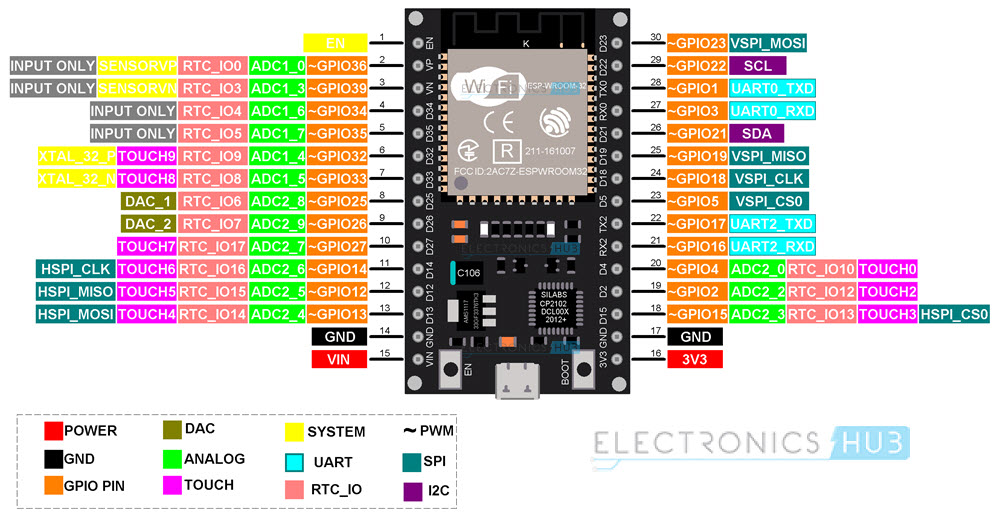
\includegraphics[width=0.8\textwidth]{img/esp32-so-do-chan-1.jpg}
    \caption{Sơ đồ chân của bo 30 chân ESP32 DevKit - Ảnh: ELECTRONICS HUB}
\end{figure}

\subsection{Hệ điều hành thời gian thực (RTOS)}

Một trong những đặc tính quan trọng trong phát triển phần mềm nhúng hiện đại là khả năng sử dụng Hệ điều hành thời gian thực (RTOS - Real-Time Operating System). Vi điều khiển ESP32 hỗ trợ chính thức hệ điều hành FreeRTOS ngay ở cấp độ nhân (Kernel).

\begin{figure}[h]
    \centering
    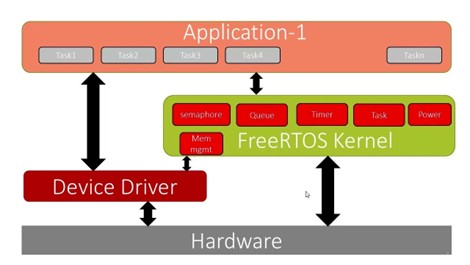
\includegraphics[width=0.8\textwidth]{img/freertos.jpg}
    \caption{Hình ảnh minh họa một dự án dùng FreeRTOS}
\end{figure}

Trong kiến trúc lập trình ``Bare-metal'' (chạy trực tiếp không có hệ điều hành), 
các lệnh được thực thi tuần tự. Khi hệ thống phải chờ đợi một tín hiệu ngoại vi 
(như chờ phản hồi HTTP từ mạng Internet), vi xử lý sẽ rơi vào trạng thái nghẽn 
(blocking), làm giảm độ nhạy của toàn bộ hệ thống. FreeRTOS giải quyết hạn chế 
này bằng cách cung cấp các cơ chế:

\begin{itemize}

\item \textbf{Đa nhiệm (Multitasking) và Lập lịch (Scheduler):} 
Chia nhỏ chương trình thành các luồng độc lập gọi là \textit{Task}. 
Bộ lập lịch sẽ phân bổ thời gian CPU (Time-slicing) cho từng Task 
dựa trên mức độ ưu tiên (Priority), tạo ra ảo giác các tác vụ đang 
chạy đồng thời.

\item \textbf{Quản lý đa lõi (Symmetric Multiprocessing):} 
Với kiến trúc lõi kép, FreeRTOS cho phép chỉ định (pin) một tác vụ 
nặng về tính toán chạy trên Core 0, trong khi các tác vụ giao tiếp 
ngoại vi theo thời gian thực chạy trên Core 1.

\item \textbf{Hàng đợi (Queue):} 
Là cấu trúc dữ liệu trung gian cho phép các Task truyền thông điệp 
(Message) cho nhau một cách an toàn, tránh tranh chấp vùng nhớ.

\end{itemize}

\section{Công nghệ nhận dạng vô tuyến RFID}

\subsection{Khái niệm và nguyên lý hoạt động}

\subsection{Công nghệ RFID}

RFID (Radio Frequency Identification) là công nghệ nhận dạng tự động sử dụng sóng vô tuyến để thu thập và truyền tải dữ liệu từ một thẻ gắn trên đối tượng cần nhận dạng.

Một hệ thống RFID cơ bản bao gồm hai thành phần chính: Đầu đọc (Reader hoặc Interrogator) và Thẻ RFID (Tag hoặc Transponder). Đầu đọc chứa bộ phát sóng vô tuyến và ăng-ten dùng để tạo ra trường điện từ và giao tiếp với thẻ. Thẻ RFID bao gồm một vi mạch (microchip) lưu trữ dữ liệu cùng với cuộn dây ăng-ten dùng để nhận và truyền tín hiệu.

Dựa vào nguồn cấp năng lượng, thẻ RFID được chia thành ba loại chính:
\begin{itemize}
    \item Thẻ chủ động (Active Tag): có nguồn pin riêng để cung cấp năng lượng cho vi mạch và phát tín hiệu.
    \item Thẻ thụ động (Passive Tag): không có pin, nhận năng lượng từ trường điện từ do đầu đọc phát ra.
    \item Thẻ bán chủ động (Semi-passive Tag): có pin để cấp nguồn cho vi mạch nhưng vẫn sử dụng tín hiệu phản xạ để giao tiếp với đầu đọc.
\end{itemize}

Để hệ thống RFID hoạt động, thẻ và đầu đọc phải làm việc trên cùng một dải tần số. Các hệ thống RFID hiện nay thường được phân thành bốn dải tần chính:
\begin{itemize}
    \item Tần số thấp (LF – Low Frequency)
    \item Tần số cao (HF – High Frequency)
    \item Tần số siêu cao (UHF – Ultra High Frequency)
    \item Tần số vi sóng (Microwave)
\end{itemize}

Nguyên lý hoạt động của thẻ RFID thụ động dựa trên định luật cảm ứng điện từ Faraday. Quá trình hoạt động diễn ra như sau:

\begin{itemize}
    \item Đầu đọc phát ra trường điện từ tần số vô tuyến thông qua ăng-ten.
    \item Khi thẻ RFID đi vào vùng phủ sóng của đầu đọc, từ thông biến thiên xuyên qua cuộn dây ăng-ten của thẻ sẽ cảm ứng ra một suất điện động.
    \item Suất điện động này được chỉnh lưu thành dòng điện một chiều (DC) để nạp vào tụ điện và cung cấp năng lượng cho vi mạch trên thẻ.
    \item Sau khi được cấp nguồn, vi mạch trong thẻ sử dụng kỹ thuật điều chế tải (Load Modulation) bằng cách thay đổi trở kháng của ăng-ten, làm biến thiên tín hiệu phản xạ về đầu đọc.
    \item Đầu đọc thu nhận sự biến thiên này và giải mã thành chuỗi dữ liệu định danh (UID) của thẻ.
\end{itemize}

\begin{figure}[h]
    \centering
    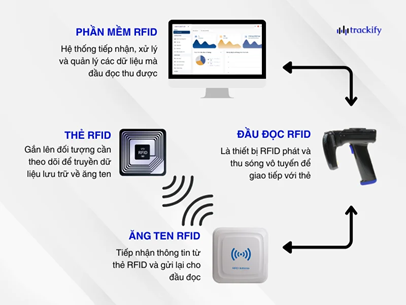
\includegraphics[width=0.7\textwidth]{img/nguyen_ly_rfid.png}
    \caption{Nguyên lý hoạt động của RFID - Ảnh: Trackify}
\end{figure}

\begin{figure}[h]
    \centering
    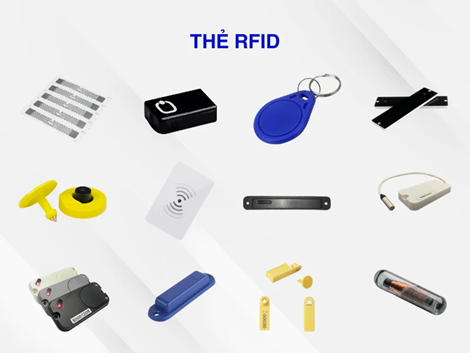
\includegraphics[width=0.7\textwidth]{img/rfid_tag.png}
    \caption{RFID tag - Ảnh: Trackify}
\end{figure}

\subsection{Đặc tính tần số và Module MFRC522}

Công nghệ RFID có thể hoạt động trên nhiều dải tần số khác nhau. Trong đó, dải tần HF (High Frequency) 13.56 MHz là tiêu chuẩn được sử dụng phổ biến nhất trên thế giới trong các ứng dụng thẻ thông minh (Smart Card), thanh toán không tiếp xúc và hệ thống kiểm soát ra vào. 

Tần số này có một số ưu điểm như tốc độ truyền dữ liệu tương đối cao (lên đến 106 kbps), hỗ trợ các cơ chế mã hóa bảo mật và ít bị ảnh hưởng bởi môi trường có chứa nước hoặc kim loại nhẹ so với một số dải tần khác.

Các hệ thống RFID hiện nay thường được phân loại dựa trên dải tần số hoạt động như trình bày trong Bảng~\ref{tab:rfid_frequency}.

\begin{table}[H]
\centering
\begin{tabular}{|c|c|c|}
\hline
\textbf{Tần số vô tuyến} & \textbf{Phân loại} & \textbf{Phạm vi truyền tín hiệu} \\
\hline
120--125 kHz & Tần số thấp & Ngắn, từ vài cm đến khoảng 1 m \\
\hline
13.56 MHz & Tần số cao & Trung bình, từ vài cm đến vài mét \\
\hline
868--928 MHz & Tần số siêu cao & Xa, có thể trên 8 m \\
\hline
2.45--5.8 GHz & Tần số vi sóng & Rất xa, có thể trên 10 m \\
\hline
\end{tabular}
\caption{Phân loại các dải tần số RFID và phạm vi truyền tín hiệu}
\label{tab:rfid_frequency}
\end{table}

Module MFRC522 là một vi mạch tích hợp cao do hãng NXP Semiconductors sản xuất, được thiết kế chuyên dụng cho các hệ thống giao tiếp RFID không tiếp xúc ở tần số 13.56 MHz. Module này tuân theo tiêu chuẩn quốc tế ISO/IEC 14443 Type A, thường được sử dụng trong các ứng dụng thẻ từ, kiểm soát truy cập và nhận dạng người dùng.

MFRC522 hỗ trợ giao tiếp với vi điều khiển thông qua nhiều giao thức như SPI, I2C và UART, trong đó giao thức SPI được sử dụng phổ biến nhất do có tốc độ truyền dữ liệu cao và khả năng tương thích tốt với các vi điều khiển như Arduino, ESP8266 và ESP32.

\begin{figure}[h]
    \centering
    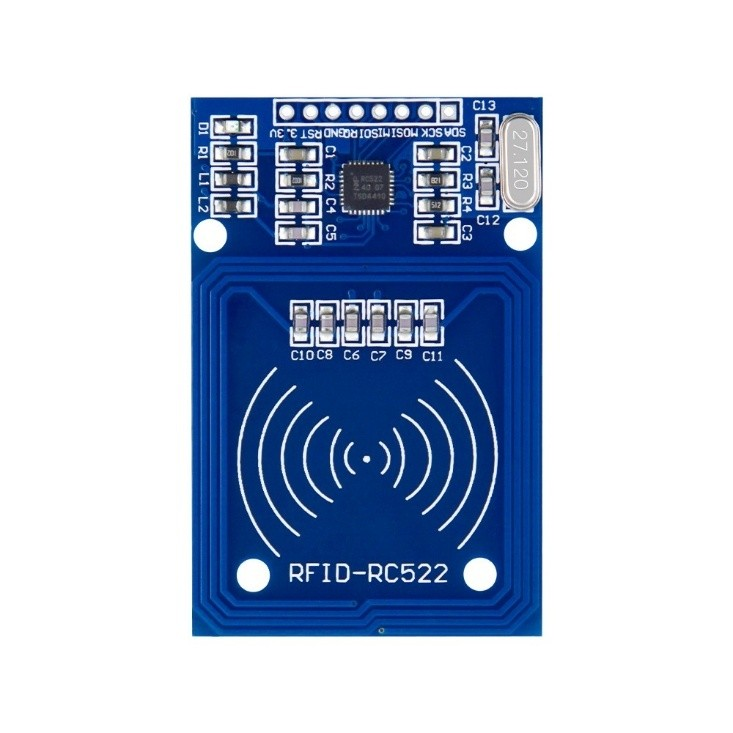
\includegraphics[width=0.5\textwidth]{img/mfrc522.jpg}
    \caption{Module MFRC522}
\end{figure}

\subsection{Cấu trúc bộ nhớ thẻ Mifare Classic 1K}

Dòng thẻ Mifare Classic 1K được trang bị bộ nhớ EEPROM với dung lượng 1024 bytes (1 KB). Bộ nhớ này được tổ chức theo cấu trúc phân tầng nhằm kiểm soát quyền truy cập dữ liệu một cách chặt chẽ.

\begin{itemize}

\item \textbf{Cấu trúc Sector:} Bộ nhớ được chia thành 16 Sector, được đánh số từ 0 đến 15.

\item \textbf{Cấu trúc Block:} Mỗi Sector bao gồm 4 Block (từ Block 0 đến Block 3), trong đó mỗi Block có dung lượng 16 bytes.

\item \textbf{Sector Trailer:} Block 3 của mỗi Sector được gọi là Sector Trailer. Block này chứa các khóa bảo mật độc lập (Key A và Key B) cùng với các bit điều kiện truy cập (Access Bits). Các thông tin này quyết định quyền đọc (Read) và ghi (Write) đối với các block dữ liệu trong cùng Sector.

\item \textbf{Manufacturer Block:} Block 0 của Sector 0 là phân vùng đặc biệt chỉ có quyền đọc (Read-only). Block này chứa các dữ liệu được nhà sản xuất lập trình sẵn từ nhà máy. Bốn byte đầu tiên của block này chính là Mã định danh duy nhất của thẻ (UID -- Unique Identifier), thường được sử dụng làm khóa định danh trong các hệ thống cơ sở dữ liệu.

\end{itemize}

\section{Các giao thức truyền thông dữ liệu}

\subsection{Giao thức ngoại vi SPI và I2C}

Tại tầng giao tiếp vật lý giữa vi điều khiển và các cảm biến, hai chuẩn truyền thông nối tiếp đồng bộ được sử dụng phổ biến nhất là:

\begin{itemize}

\item \textbf{SPI (Serial Peripheral Interface):} 
Là chuẩn truyền thông song công toàn phần (Full-duplex), cho phép truyền và nhận dữ liệu đồng thời với tốc độ cao (có thể đạt tới hàng chục Mbps). 
SPI hoạt động theo mô hình \textit{Master -- Slave} thông qua bốn đường tín hiệu chính:

\begin{itemize}
\item \texttt{SCK} (Serial Clock): Xung nhịp đồng bộ do thiết bị Master tạo ra.
\item \texttt{MOSI} (Master Out Slave In): Đường truyền dữ liệu từ Master đến Slave.
\item \texttt{MISO} (Master In Slave Out): Đường truyền dữ liệu từ Slave về Master.
\item \texttt{SS/CS} (Slave Select / Chip Select): Chân dùng để chọn thiết bị Slave cần giao tiếp.
\end{itemize}

Nhờ băng thông truyền dữ liệu lớn và độ trễ thấp, SPI thường được sử dụng để giao tiếp với các module yêu cầu tốc độ cao như module đọc thẻ RFID.

\item \textbf{I2C (Inter-Integrated Circuit):} 
Là giao thức truyền thông bán song công (Half-duplex), hoạt động theo cấu trúc bus với hai đường tín hiệu chính:

\begin{itemize}
\item \texttt{SDA} (Serial Data): Đường truyền dữ liệu.
\item \texttt{SCL} (Serial Clock): Đường xung nhịp đồng bộ.
\end{itemize}

I2C cho phép kết nối nhiều thiết bị trên cùng một bus nhờ cơ chế địa chỉ hóa 7-bit hoặc 10-bit. 
Giao thức này thường được sử dụng cho các thiết bị ngoại vi có tốc độ truyền thấp như màn hình LCD, cảm biến nhiệt độ hoặc module RTC, giúp giảm số lượng chân GPIO cần sử dụng trên vi điều khiển.

\end{itemize}

\begin{figure}[h]
    \centering
    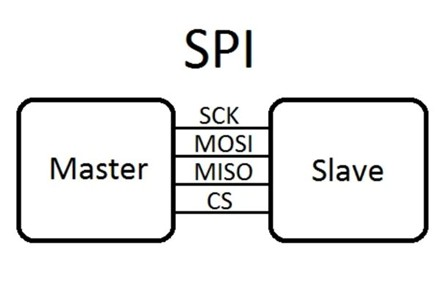
\includegraphics[width=0.5\textwidth]{img/spi.jpg}
    \caption{Hình ảnh minh họa giao thức SPI}
\end{figure}

\subsection{Giao thức HTTP và Kiến trúc RESTful API}

Trong mạng Internet, giao thức \textbf{HTTP (Hypertext Transfer Protocol)} là nền tảng của truyền thông dữ liệu giữa các hệ thống. 
Để xây dựng các hệ thống phân tán, chuẩn kiến trúc \textbf{REST (Representational State Transfer)} được sử dụng rộng rãi để thiết kế các \textbf{API (Application Programming Interface)}.

RESTful API hoạt động dựa trên mô hình \textit{Client -- Server} và có đặc tính \textbf{phi trạng thái (Stateless)}. 
Điều này có nghĩa là mỗi yêu cầu (Request) từ Client gửi đến Server phải chứa đầy đủ thông tin cần thiết để Server xử lý. 
Server sẽ không lưu trữ ngữ cảnh của các yêu cầu trước đó.

Các phương thức HTTP (\textit{HTTP Methods}) định nghĩa loại hành động mà Client muốn thực hiện:

\begin{itemize}

\item \texttt{GET}: 
Được sử dụng để truy xuất dữ liệu từ máy chủ (chỉ đọc thông tin, không làm thay đổi dữ liệu trên Server).

\item \texttt{POST}: 
Được sử dụng để gửi dữ liệu mới từ Client đến Server nhằm xử lý hoặc lưu trữ vào cơ sở dữ liệu.

\item \textbf{Mã trạng thái (Status Codes):} 
Server phản hồi kết quả xử lý cho Client thông qua các mã trạng thái chuẩn hóa, ví dụ:

\begin{itemize}
\item \texttt{200 OK}: Yêu cầu được xử lý thành công.
\item \texttt{400 Bad Request}: Dữ liệu yêu cầu không hợp lệ.
\item \texttt{401 Unauthorized}: Yêu cầu cần xác thực nhưng chưa được cung cấp thông tin xác thực hợp lệ.
\item \texttt{500 Internal Server Error}: Lỗi xảy ra ở phía máy chủ.
\end{itemize}

\end{itemize}

\subsection{Định dạng dữ liệu JSON}

Để trao đổi thông điệp giữa các nền tảng lập trình khác nhau như C++, Python và JavaScript, hệ thống sử dụng định dạng dữ liệu trung gian \textbf{JSON (JavaScript Object Notation)}. JSON là một chuẩn mở có định dạng văn bản nhẹ, lưu trữ dữ liệu dưới dạng cấu trúc \textit{Khóa -- Giá trị (Key--Value)} và \textit{Mảng (Array)}.

Quá trình làm việc với JSON bao gồm hai bước chính:

\begin{itemize}

\item \textbf{Serialization (Tuần tự hóa):} 
Biến đổi cấu trúc dữ liệu trong bộ nhớ RAM của thiết bị thành một chuỗi ký tự JSON dạng văn bản để gửi qua mạng.

\item \textbf{Deserialization (Giải tuần tự hóa):} 
Phân tích cú pháp (Parse) chuỗi JSON nhận được từ mạng để tái tạo lại cấu trúc dữ liệu ban đầu vào bộ nhớ của thiết bị.

\end{itemize}

\section{Công nghệ Web và cơ sở dữ liệu}

\subsection{Hệ quản trị cơ sở dữ liệu quan hệ (RDBMS) và tính chất ACID}

Cơ sở dữ liệu là nơi lưu trữ và quản lý thông tin một cách bền vững. Các ứng dụng phần mềm yêu cầu tính toàn vẹn dữ liệu cao thường sử dụng \textbf{Hệ quản trị Cơ sở dữ liệu Quan hệ (RDBMS -- Relational Database Management System)} như PostgreSQL hoặc MySQL.

Trong RDBMS, dữ liệu được tổ chức dưới dạng các \textbf{bảng (Tables)}. Các bảng được liên kết với nhau thông qua \textbf{Khóa chính (Primary Key)} và \textbf{Khóa ngoại (Foreign Key)}, nhằm đảm bảo \textbf{tính toàn vẹn tham chiếu (Referential Integrity)} và ngăn chặn việc tạo ra các bản ghi mồ côi (Orphan Records).

Một hệ quản trị cơ sở dữ liệu quan hệ phải tuân thủ bốn thuộc tính quan trọng của giao dịch, được gọi là \textbf{ACID}:

\begin{itemize}

\item \textbf{Atomicity (Tính nguyên tử):} 
Một giao dịch có thể bao gồm nhiều thao tác. Nếu bất kỳ thao tác nào thất bại, toàn bộ giao dịch sẽ bị hủy bỏ (Rollback) và cơ sở dữ liệu trở về trạng thái ban đầu.

\item \textbf{Consistency (Tính nhất quán):} 
Cơ sở dữ liệu phải chuyển từ một trạng thái hợp lệ sang một trạng thái hợp lệ khác, tuân thủ tất cả các ràng buộc đã được định nghĩa.

\item \textbf{Isolation (Tính cô lập):} 
Các giao dịch thực thi đồng thời không được phép ảnh hưởng đến dữ liệu đang được xử lý của nhau.

\item \textbf{Durability (Tính bền vững):} 
Sau khi một giao dịch được xác nhận (Committed), dữ liệu phải được lưu trữ vĩnh viễn trên thiết bị lưu trữ.

\end{itemize}

\begin{figure}[h]
    \centering
    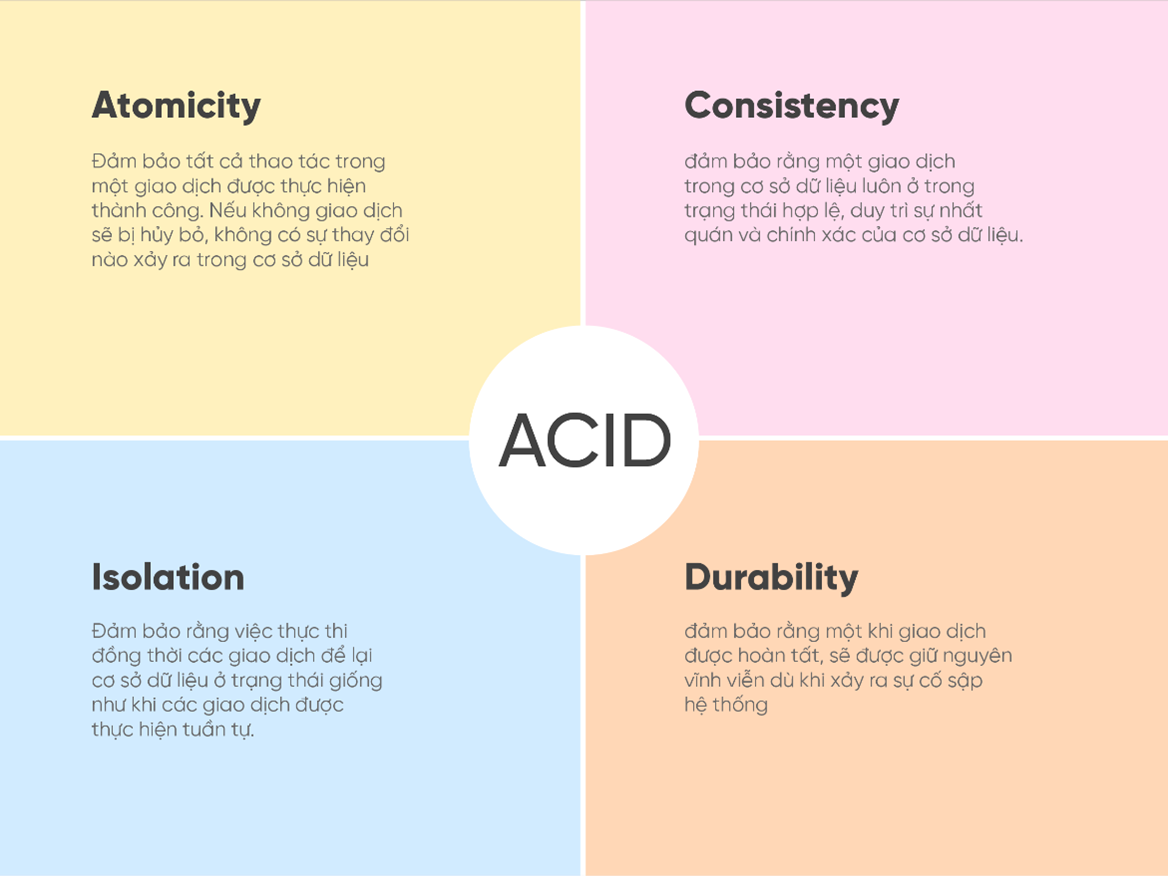
\includegraphics[width=0.7\textwidth]{img/tinh_chat_acid.png}
    \caption{Bốn tính chất của ACID trong giao dịch cơ sở dữ liệu - Ảnh: ScyllaDB}
\end{figure}

\subsection{Khung phần mềm Web (Web Framework)}

Phần mềm máy chủ (\textit{Backend}) đóng vai trò trung gian xử lý logic giữa thiết bị đầu cuối và cơ sở dữ liệu. Trong hệ sinh thái ngôn ngữ Python, các Web Framework hiện đại như \textbf{FastAPI} được xây dựng dựa trên chuẩn \textbf{ASGI (Asynchronous Server Gateway Interface)}.

Sự khác biệt lớn nhất của các framework hiện đại là khả năng lập trình \textbf{bất đồng bộ (Asynchronous I/O)}. Khi máy chủ nhận một truy vấn cần thời gian để xử lý (ví dụ: truy xuất dữ liệu từ ổ đĩa hoặc chờ phản hồi từ cơ sở dữ liệu), thay vì giữ CPU ở trạng thái chờ đợi vô ích (\textit{Blocking}), framework sẽ giải phóng luồng đó để CPU có thể phục vụ các yêu cầu khác từ các Client.

Nhờ cơ chế này, máy chủ có thể xử lý hàng chục nghìn kết nối đồng thời (\textit{High Concurrency}) với mức tiêu thụ tài nguyên phần cứng rất thấp.

\subsection{Xung đột luồng (Race Condition) và Đồng bộ hóa (Synchronization)}

Trong khoa học máy tính, các hệ thống đa luồng (\textit{Multithreading}) luôn phải đối mặt với bài toán tương tranh và hiện tượng \textbf{Race Condition}.

\textbf{Hiện tượng Race Condition:}  
Xảy ra khi hai hoặc nhiều luồng xử lý cùng chia sẻ và sửa đổi một tài nguyên chung (\textit{Shared Resource} -- ví dụ: một bản ghi trong cơ sở dữ liệu) tại gần như cùng một thời điểm. Do CPU thực thi các lệnh đọc/ghi xen kẽ nhau một cách không xác định, dữ liệu cuối cùng được lưu trữ có thể phụ thuộc vào thứ tự thực thi của các luồng, dẫn đến sự sai lệch dữ liệu (\textit{Data Inconsistency}).

\textbf{Cơ chế đồng bộ hóa bằng khóa (Mutex Lock):}

Để ngăn chặn xung đột luồng, hệ điều hành và các ngôn ngữ lập trình cung cấp cơ chế \textbf{Mutual Exclusion Lock (Mutex)}. Đoạn mã thực hiện việc truy cập tài nguyên chung được gọi là \textbf{Khu vực găng (Critical Section)}.

Cơ chế Mutex quy định:

\begin{itemize}

\item Tại một thời điểm, chỉ có duy nhất một luồng được phép giữ khóa và truy cập vào khu vực găng.

\item Các luồng khác khi đến sau phải chuyển sang trạng thái chờ (\textit{Wait}) cho đến khi khóa được giải phóng.

\item Sau khi hoàn tất thao tác với tài nguyên chung, luồng đang giữ khóa sẽ thực hiện thao tác \textit{Release Lock} để cho phép luồng tiếp theo truy cập.

\end{itemize}

Cơ chế này giúp loại bỏ hoàn toàn nguy cơ ghi đè dữ liệu và đảm bảo tính nhất quán cho hệ thống cơ sở dữ liệu.

\chapter{THIẾT KẾ HỆ THỐNG}

\section{Phân tích yêu cầu và sơ đồ khối kiến trúc hệ thống}

\subsection{Phân tích yêu cầu hệ thống}

Để đáp ứng điều kiện vận hành tại môi trường lớp học thực tế có quy mô lớn, hệ thống cần thỏa mãn các yêu cầu kỹ thuật sau:

\begin{itemize}

\item \textbf{Yêu cầu chức năng:} 
Thiết bị phải có khả năng nhận diện thẻ RFID và phản hồi trạng thái cho người dùng thông qua âm thanh, đèn báo hoặc màn hình LCD. Hệ thống phải tự động xác định ca học hiện tại dựa trên thời gian thực. Đồng thời, giảng viên có thể theo dõi, quản lý điểm danh và xuất báo cáo thông qua giao diện Web.

\item \textbf{Yêu cầu phi chức năng (Hiệu năng):}

\begin{itemize}

\item Độ trễ phản hồi tại thiết bị biên (\textit{Edge latency}) khi sinh viên quẹt thẻ phải nhỏ hơn 0.5 giây để tránh tình trạng ùn tắc tại lớp học.

\item Hệ thống máy chủ phải có khả năng xử lý nhiều truy vấn đồng thời (\textit{Concurrency}) mà không xảy ra tình trạng mất mát hoặc sai lệch dữ liệu khi nhiều sinh viên quẹt thẻ cùng lúc.

\item Tối ưu hóa băng thông truyền tải và tiết kiệm tài nguyên bộ nhớ (\textit{SRAM}) của vi điều khiển.

\end{itemize}

\end{itemize}

\subsection{Sơ đồ khối tổng quát}

Hệ thống được thiết kế theo kiến trúc \textbf{Edge-to-Cloud}, bao gồm bốn phân hệ chính hoạt động liên kết với nhau thông qua mạng Internet:

\begin{itemize}

\item \textbf{Khối thiết bị biên (IoT Edge Node -- ESP32):} 
Là thiết bị phần cứng được lắp đặt tại phòng học. Khối này có nhiệm vụ thu thập tín hiệu vô tuyến từ thẻ RFID, lưu trữ tạm thời danh sách sinh viên trong bộ nhớ đệm (\textit{Cache}) và hiển thị thông tin tương tác với người dùng thông qua màn hình LCD 1602.

\item \textbf{Khối máy chủ ứng dụng (Backend API Server):} 
Được xây dựng bằng framework \textbf{FastAPI} trên nền tảng Python. Khối này đóng vai trò là trung tâm xử lý logic của hệ thống, tiếp nhận các yêu cầu HTTP từ thiết bị ESP32, thực hiện thuật toán xác định ca học dựa trên thời gian thực và xử lý đồng bộ luồng (\textit{Thread Synchronization}) trước khi ghi dữ liệu vào cơ sở dữ liệu.

\item \textbf{Khối cơ sở dữ liệu (Database Layer):} 
Sử dụng hệ quản trị cơ sở dữ liệu quan hệ \textbf{PostgreSQL} triển khai trên nền tảng đám mây \textbf{Supabase}. Thành phần này có nhiệm vụ lưu trữ bền vững mọi dữ liệu của hệ thống như thông tin sinh viên, thời khóa biểu và nhật ký điểm danh.

\item \textbf{Khối giao diện quản trị (Web Client):} 
Là ứng dụng Web dành cho giảng viên. Giao diện này giao tiếp trực tiếp với Backend API để theo dõi trạng thái lớp học, quản lý dữ liệu điểm danh và xuất báo cáo.

\end{itemize}

\begin{figure}[H]
    \centering
    \includegraphics[width=1\textwidth]{img/so_do_khoi.png}
    \caption{Sơ đồ khối tổng quát của hệ thống}
\end{figure}

\subsection{Kiến trúc bộ đệm thông minh}

Để thỏa mãn yêu cầu về thời gian phản hồi rất thấp (< 0.5s) và khắc phục giới hạn bộ nhớ SRAM của ESP32 (520 KB), đề tài thiết kế một cơ chế đồng bộ dữ liệu động có tên \textbf{Smart Edge Caching}.

Thay vì lưu tĩnh toàn bộ danh sách sinh viên của trường vào chương trình, thiết bị hoạt động theo nguyên lý sau:

\begin{itemize}

\item \textbf{Đồng bộ định kỳ:}

Khi khởi động và cứ mỗi 30 phút một lần (\texttt{UPDATE\_LIST\_INTERVAL = 1.800.000 ms}), ESP32 chủ động gửi một yêu cầu HTTP \textbf{GET} tới API \texttt{/api/students/\{device\_id\}} của máy chủ.

\item \textbf{Máy chủ suy luận:}

Máy chủ lấy thời gian hệ thống hiện tại (chuẩn múi giờ UTC+7), kết hợp với mã phòng học tương ứng của \texttt{device\_id} để dò tìm trong bảng \textit{Thời khóa biểu}. Khi tìm thấy lớp học đang diễn ra, máy chủ trả về một mảng dữ liệu định dạng \textbf{JSON} chứa danh sách sinh viên của lớp đó.

\item \textbf{Xử lý Offline tại thiết bị biên:}

ESP32 phân tích cú pháp chuỗi JSON và cập nhật vào mảng cấu trúc (\textit{Struct}) \texttt{students} với giới hạn tối đa 100 sinh viên. Khi sinh viên quẹt thẻ, vi điều khiển chỉ cần vài mili-giây để duyệt mảng dữ liệu trong RAM và hiển thị kết quả lên màn hình LCD, qua đó loại bỏ hoàn toàn độ trễ do đường truyền Internet.

\end{itemize}

\section{Thiết kế cơ sở dữ liệu}

Cơ sở dữ liệu của hệ thống được thiết kế trên hệ quản trị \textbf{PostgreSQL} (triển khai trên nền tảng Supabase) và tuân thủ nghiêm ngặt \textbf{dạng chuẩn hóa thứ ba (3NF)} nhằm loại bỏ sự dư thừa dữ liệu và đảm bảo tính toàn vẹn tham chiếu giữa các bảng.

\subsection{Sơ đồ quan hệ thực thể (ERD)}

Mô hình dữ liệu của hệ thống bao gồm các thực thể chính sau:

\begin{itemize}

\item \textbf{Sinh viên (Students)}

\item \textbf{Lớp học (Classes)}

\item \textbf{Thiết bị (Devices)}

\item \textbf{Nhật ký điểm danh (Attendance Logs)}

\item \textbf{Quản trị viên (Admin Users)}

\item \textbf{Danh sách lớp (Class Lists)}

\end{itemize}

\begin{figure}[htbp]
    \centering
    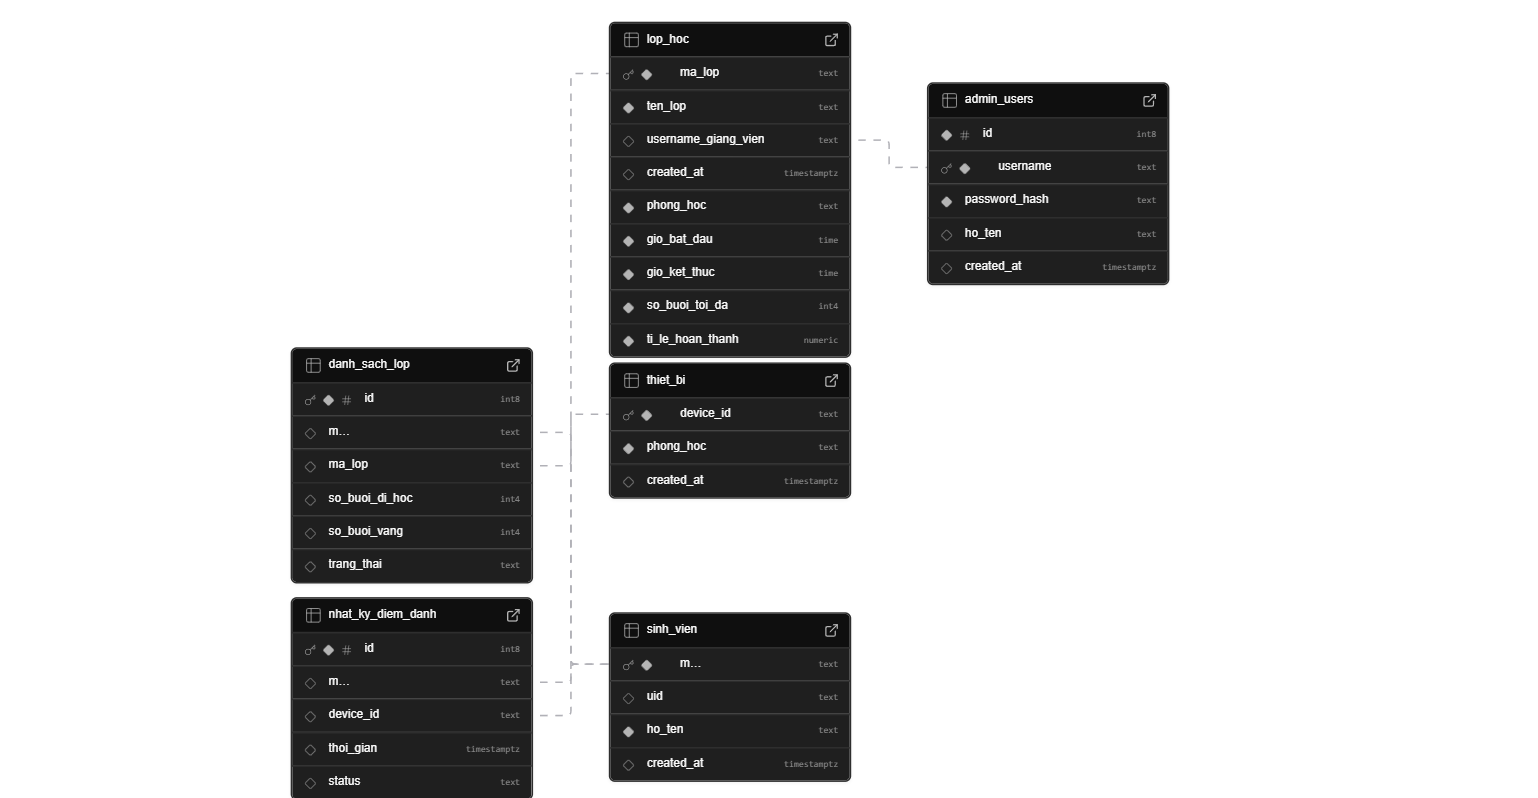
\includegraphics[width=1.2\textwidth]{img/data_schema.png}
    \caption{Sơ đồ quan hệ thực thể (ERD)}
\end{figure}
\FloatBarrier

\subsection{Đặc tả chi tiết các bảng dữ liệu}

\textbf{Bảng 1: admin\_users (Quản lý tài khoản Giảng viên / Quản trị viên)}

Bảng này lưu trữ thông tin xác thực của các giảng viên để đăng nhập vào hệ thống Web Dashboard.

\begin{table}[H]
\centering
\caption{Bảng admin\_users}
\begin{tabularx}{\textwidth}{|l|l|l|X|}
\hline
\textbf{Tên trường} & \textbf{Kiểu dữ liệu} & \textbf{Ràng buộc} & \textbf{Mô tả chức năng} \\ \hline
admin\_users & TEXT & PRIMARY KEY & Tên đăng nhập của giảng viên \\ \hline
id & BIGINT & IDENTITY & Khóa phụ tự động tăng định danh duy nhất \\ \hline
password\_hash & TEXT & NOT NULL & Chuỗi mật khẩu đã được băm (hashing) bằng thuật toán bcrypt để bảo mật \\ \hline
ho\_ten & TEXT &  & Họ và tên đầy đủ của giảng viên \\ \hline
created\_at & TIMESTAMPTZ & DEFAULT now() & Mốc thời gian hệ thống tạo tài khoản này \\ \hline
\end{tabularx}
\end{table}

\textbf{Bảng 2: sinh\_vien (Quản lý thông tin định danh sinh viên)}

Bảng chứa dữ liệu tĩnh của người học, được sử dụng để đối chiếu với thẻ RFID.

\begin{table}[H]
\centering
\caption{Bảng sinh\_vien}
\begin{tabularx}{\textwidth}{|l|l|l|X|}
\hline
\textbf{Tên trường} & \textbf{Kiểu dữ liệu} & \textbf{Ràng buộc} & \textbf{Mô tả chức năng} \\ \hline
mssv & TEXT &  & Mã số sinh viên \\ \hline
uid & TEXT &  & Mã UID vật lý của thẻ RFID gắn với sinh viên này \\ \hline
ho\_ten & TEXT & NOT NULL & Họ và tên đầy đủ của sinh viên \\ \hline
created\_at & TIMESTAMPTZ & DEFAULT now() & Mốc thời gian nạp dữ liệu sinh viên vào hệ thống \\ \hline
\end{tabularx}
\end{table}

\textbf{Bảng 3: thiet\_bi (Quản lý thiết bị IoT đầu cuối)}

Bảng này đóng vai trò ánh xạ địa chỉ logic của mạch ESP32 với không gian vật lý.

\begin{table}[H]
\centering
\caption{Bảng thiet\_bi}
\begin{tabularx}{\textwidth}{|l|l|l|X|}
\hline
\textbf{Tên trường} & \textbf{Kiểu dữ liệu} & \textbf{Ràng buộc} & \textbf{Mô tả chức năng} \\ \hline
device\_id & TEXT & PRIMARY KEY & Mã định danh phần cứng \\ \hline
phong\_hoc & TEXT & NOT NULL & Tên phòng học vật lý được lắp đặt thiết bị này \\ \hline
created\_at & TIMESTAMPTZ & DEFAULT now() & Thời gian khai báo thiết bị lên hệ thống \\ \hline
\end{tabularx}
\end{table}

\textbf{Bảng 4: lop\_hoc (Cấu hình Thời khóa biểu và Học phần)}

Đây là bảng cốt lõi chứa cấu hình thời gian và không gian, giúp Backend tự động nội suy ca học khi thiết bị gửi dữ liệu lên.

\begin{table}[H]
\centering
\renewcommand{\arraystretch}{1.3}
\caption{Bảng \textit{lop\_hoc}}
\begin{tabularx}{\textwidth}{|c|c|c|X|}
\hline
\textbf{Tên trường} & \textbf{Kiểu dữ liệu} & \textbf{Ràng buộc} & \textbf{Mô tả chức năng} \\ 
\hline
ma\_lop & TEXT & PRIMARY KEY & Mã lớp học phần duy nhất trong hệ thống. \\ 
\hline
ten\_lop & TEXT & NOT NULL & Tên môn học được hiển thị trên giao diện Web Dashboard. \\ 
\hline
username\_giang\_vien & TEXT & FOREIGN KEY & Liên kết với bảng \textit{admin\_users} để xác định giảng viên quản lý lớp học phần này. \\ 
\hline
phong\_hoc & TEXT & NOT NULL & Tên phòng học nơi môn học diễn ra, được đối chiếu với bảng \textit{thiet\_bi} để xác định thiết bị điểm danh. \\ 
\hline
gio\_bat\_dau & TIME & NOT NULL & Thời điểm bắt đầu ca học theo thời khóa biểu. \\ 
\hline
gio\_ket\_thuc & TIME & NOT NULL & Thời điểm kết thúc ca học. \\ 
\hline
so\_buoi\_toi\_da & INTEGER & NOT NULL & Tổng số buổi học của môn theo đề cương đào tạo. \\ 
\hline
ti\_le\_hoan\_thanh & NUMERIC & NOT NULL & Tỷ lệ số buổi tham gia tối thiểu để sinh viên đủ điều kiện dự thi. \\ 
\hline
created\_at & TIMESTAMPTZ & DEFAULT now() & Thời điểm hệ thống tạo bản ghi cấu hình lớp học trong cơ sở dữ liệu. \\ 
\hline
\end{tabularx}
\end{table}


\textbf{Bảng 5: danh\_sach\_lop (Quản lý tiến độ điểm danh)}

Bảng trung gian giải quyết mối quan hệ Nhiều - Nhiều (n-n) giữa Sinh viên và Lớp học.

\begin{table}[H]
\centering
\caption{Bảng danh\_sach\_lop}
\begin{tabularx}{\textwidth}{|l|l|l|X|}
\hline
\textbf{Tên trường} & \textbf{Kiểu dữ liệu} & \textbf{Ràng buộc} & \textbf{Mô tả chức năng} \\ \hline
id & BIGINT & PRIMARY KEY, IDENTITY & Khóa định danh tự động tăng \\ \hline
mssv & TEXT & FOREIGN KEY & Liên kết với bảng sinh\_vien \\ \hline
ma\_lop & TEXT & FOREIGN KEY & Liên kết với bảng lop\_hoc \\ \hline
so\_buoi\_di\_hoc & INTEGER & DEFAULT 0 & Bộ đếm số buổi điểm danh thành công \\ \hline
so\_buoi\_vang & INTEGER & DEFAULT 0 & Bộ đếm số buổi vắng mặt \\ \hline
trang\_thai & TEXT & DEFAULT 'Chưa được thi' & Trạng thái cảnh báo học vụ dựa trên tỷ lệ chuyên cần \\ \hline
\end{tabularx}
\end{table}

\subsection{Bảng 6: nhat\_ky\_diem\_danh}

Bảng \texttt{nhat\_ky\_diem\_danh} lưu trữ toàn bộ lịch sử tương tác giữa thẻ RFID và thiết bị IoT. 
Dữ liệu này phục vụ cho mục đích kiểm toán hệ thống, dò lỗi trong quá trình vận hành và trích xuất 
các báo cáo thống kê chuyên cần của sinh viên.

\begin{table}[H]
\centering
\caption{Bảng nhat\_ky\_diem\_danh}
\begin{tabularx}{\textwidth}{|l|l|l|X|}
\hline
\textbf{Tên trường} & \textbf{Kiểu dữ liệu} & \textbf{Ràng buộc} & \textbf{Mô tả chức năng} \\
\hline
id & BIGINT & PRIMARY KEY, IDENTITY & Khóa chính tự động tăng mỗi khi có giao dịch điểm danh mới được ghi nhận. \\
\hline
mssv & TEXT & FOREIGN KEY & Mã số sinh viên thực hiện quẹt thẻ. Trường này có thể để trống nếu hệ thống phát hiện thẻ lạ chưa được đăng ký. \\
\hline
device\_id & TEXT & FOREIGN KEY & Mã định danh của thiết bị IoT nhận tín hiệu quẹt thẻ, liên kết với bảng \texttt{thiet\_bi}. \\
\hline
thoi\_gian & TIMESTAMPTZ & DEFAULT now() & Thời điểm chính xác khi hệ thống ghi nhận giao dịch điểm danh từ thiết bị. \\
\hline
status & TEXT & DEFAULT 'Present' & Trạng thái điểm danh của giao dịch. Có thể là \texttt{Present} (hợp lệ), \texttt{Guest} (thẻ lạ) hoặc \texttt{Manual Update} khi giảng viên cập nhật thủ công trên hệ thống Web. \\
\hline
\end{tabularx}
\label{bang:nhatky_diemdanh}
\end{table}

\section{Thiết kế Giải thuật và Logic điều khiển}

\subsection{Giải thuật xử lý tại thiết bị biên (Firmware ESP32)}

Chương trình nạp trên ESP32 được xây dựng dựa trên nguyên lý đa luồng 
(Multithreading) của hệ điều hành FreeRTOS. Vi điều khiển sử dụng hàng đợi 
\texttt{QueueHandle\_t uploadQueue} để giao tiếp giữa hai nhân xử lý (Core 0 và Core 1).

\textbf{Luồng nghiệp vụ chính (Loop -- Core 1):}

\begin{itemize}

\item Bắt đầu chu kỳ, sử dụng hàm \texttt{millis()} để kiểm tra độ lệch thời gian so với 
\texttt{lastUpdateListMs}. Nếu vượt quá 30 phút, hệ thống tạm ngưng để gọi API 
cập nhật lại danh sách sinh viên vào mảng \texttt{students[]}.

\item Kiểm tra bộ đệm UART của tín hiệu RFID. Khi phát hiện thẻ trong vùng đọc,
thiết bị sẽ trích xuất chuỗi UID của thẻ.

\item Áp dụng thuật toán chống dội thẻ (Anti-bounce): so sánh UID vừa quét với 
\texttt{lastUid} và kiểm tra điều kiện 
\texttt{millis() - lastScanMs < 2000}. 
Nếu điều kiện đúng, chu kỳ xử lý sẽ bị hủy để tránh ghi nhận nhiều lần trong vòng 2 giây.

\item Thực hiện vòng lặp \texttt{for} để đối chiếu UID với danh sách sinh viên 
\texttt{students[]} trong bộ nhớ RAM.

\begin{itemize}

\item Nếu tìm thấy UID hợp lệ: bật đèn xanh, kích hoạt relay, phát còi ngắn 
và hiển thị tên sinh viên trên màn hình LCD.

\item Nếu không tìm thấy: bật đèn đỏ, phát còi dài và hiển thị thông báo 
``UNKNOWN CARD''.

\end{itemize}

\item Khởi tạo cấu trúc dữ liệu \texttt{UploadData} gồm UID và thời gian 
Epoch. Gói dữ liệu được gửi vào hàng đợi \texttt{uploadQueue} bằng hàm 
\texttt{xQueueSend}. Hàm này có thời gian chờ tối đa 1000ms để tránh mất gói tin 
khi luồng mạng đang bận.

\item Xóa màn hình LCD và đưa thiết bị trở về trạng thái 
``Ready to Scan'' để chờ sinh viên tiếp theo.

\end{itemize}

\textbf{Luồng truyền tải mạng (TaskUpload -- Core 0):}

\begin{itemize}

\item Luồng này hoạt động độc lập bằng vòng lặp vô hạn \texttt{while(true)}.

\item Sử dụng hàm \texttt{xQueueReceive} để chờ dữ liệu từ hàng đợi.
Nếu hàng đợi rỗng, luồng sẽ tự động chuyển sang trạng thái \textit{Block}
để không tiêu tốn tài nguyên CPU.

\item Khi nhận được dữ liệu, hệ thống tạo đối tượng 
\texttt{StaticJsonDocument} để đóng gói các trường:
\texttt{uid}, \texttt{device\_id}, và \texttt{time\_scan}.

\item Thư viện \texttt{HTTPClient} được sử dụng để thiết lập kết nối TCP
tới máy chủ Backend. Gói tin JSON được gửi thông qua phương thức POST
với Header \texttt{application/json}.

\item Sau khi gửi dữ liệu, hệ thống đọc mã phản hồi HTTP và đóng kết nối,
đồng thời giải phóng bộ nhớ tạm.

\end{itemize}

\subsection{Giải thuật đồng bộ và xử lý logic tại máy chủ Backend}

API \texttt{POST /api/attendance} trên máy chủ FastAPI là nơi thực thi
các logic quan trọng của hệ thống. Để tránh hiện tượng xung đột luồng
(\textit{Race Condition}) khi nhiều thiết bị gửi yêu cầu cùng lúc,
hệ thống sử dụng cơ chế khóa loại trừ tương hỗ (\textit{Mutex Lock})
thông qua đối tượng:

\begin{verbatim}
db_lock = threading.Lock()
\end{verbatim}

\textbf{Tiến trình xử lý trong vùng găng (Critical Section):}

\begin{itemize}

\item Nhận dữ liệu JSON từ ESP32 và kích hoạt khối lệnh 
\texttt{with db\_lock}. Trong thời gian này, toàn bộ truy cập cơ sở dữ liệu
được khóa để đảm bảo tính nhất quán.

\item Truy vấn bảng \texttt{thiet\_bi} để xác định 
\texttt{phong\_hoc} dựa trên \texttt{device\_id}. 
Nếu không tìm thấy thiết bị, hệ thống trả về lỗi HTTP 400.

\item Chuyển đổi \texttt{time\_scan} sang đối tượng 
\texttt{DateTime} theo múi giờ Việt Nam (UTC+7). Sau đó truy vấn bảng
\texttt{lop\_hoc} với ba điều kiện:
\begin{itemize}
\item Phòng học trùng khớp
\item \texttt{gio\_bat\_dau <= time\_scan}
\item \texttt{gio\_ket\_thuc >= time\_scan}
\end{itemize}

Nếu không tìm thấy lớp học phù hợp, hệ thống trả về lỗi HTTP 400.

\item Đối chiếu UID với bảng \texttt{sinh\_vien} để xác định mã sinh viên
(\texttt{mssv}).

\item Nếu sinh viên thuộc lớp học hiện tại, hệ thống cập nhật
\texttt{so\_buoi\_di\_hoc = N + 1} và gán trạng thái 
\texttt{status\_log = "Present"}.
Nếu không thuộc lớp, trạng thái được gán là \texttt{"Guest"}.

\item Ghi một bản ghi mới vào bảng \texttt{nhat\_ky\_diem\_danh}
để lưu lại lịch sử giao dịch.

\item Trả về phản hồi thành công:

\begin{verbatim}
{"status": "success"}
\end{verbatim}

Sau khi hoàn tất, khóa \texttt{db\_lock} được giải phóng để
các yêu cầu tiếp theo có thể tiếp tục xử lý.

\end{itemize}

\section{Thiết kế Giao tiếp API}

\begin{longtable}{|p{3.5cm}|p{2cm}|p{4cm}|p{6cm}|}
\caption{Danh sách các API Endpoints trong hệ thống} \\

\hline
\textbf{Endpoint / Đường dẫn} & \textbf{Phương thức} & \textbf{Dữ liệu đầu vào} & \textbf{Chức năng chi tiết} \\ 
\hline
\endfirsthead

\hline
\textbf{Endpoint / Đường dẫn} & \textbf{Phương thức} & \textbf{Dữ liệu đầu vào} & \textbf{Chức năng chi tiết} \\ 
\hline
\endhead

/api\allowbreak/students\allowbreak/\{device\_id\} & GET &
Tham số đường dẫn: device\_id &
Hệ thống kiểm tra ca học đang diễn ra tại thiết bị tương ứng và trả về mảng JSON chứa tối đa 100 sinh viên (UID, MSSV, Họ tên) để ESP32 lưu đệm. \\ \hline

/api/attendance & POST &
JSON Body: \{uid, device\_id, time\_scan\} &
Nhận dữ liệu sinh viên quẹt thẻ từ thiết bị. Hệ thống thực hiện kiểm tra logic điểm danh, xử lý đồng bộ luồng và cập nhật dữ liệu chuyên cần vào cơ sở dữ liệu. \\ \hline

/token & POST &
Form Data: username, password &
Tiếp nhận thông tin đăng nhập của giảng viên, kiểm tra mật khẩu đã băm bằng bcrypt và trả về chuỗi JSON Web Token (JWT) có thời hạn 30 phút. \\ \hline

/my-classes & GET &
Header Authorization: Bearer <token> &
Giải mã JWT để xác định danh tính giảng viên và trả về danh sách các lớp học mà giảng viên đang phụ trách. \\ \hline

/stats & GET &
Query Parameter: ?ma\_lop=... &
Truy xuất dữ liệu thống kê điểm danh của một lớp học cụ thể từ cơ sở dữ liệu để hiển thị trên giao diện Web quản trị. \\ \hline

/update-attendance & POST &
JSON Body: \{mssv, ma\_lop, action\} &
Cho phép giảng viên điều chỉnh thủ công số buổi điểm danh của sinh viên (cộng hoặc trừ) trong trường hợp sinh viên quên thẻ hoặc xảy ra sai sót. \\ \hline

/export & GET &
Query Parameter: ?ma\_lop=... &
Hệ thống sử dụng thư viện pandas để chuyển đổi dữ liệu điểm danh thành tệp Excel (.xlsx) và trả về cho trình duyệt tải xuống. \\ \hline

\end{longtable}

\section{Thiết kế Giao diện Web Quản trị (Frontend)} 

Giao diện ứng dụng Web được thiết kế dành riêng cho giảng viên và nhân viên quản lý đào tạo. Hệ thống hướng đến phong cách giao diện hiện đại, sử dụng hiệu ứng kính mờ (Glassmorphism) nhằm tạo cảm giác trực quan, dễ sử dụng và phù hợp với xu hướng thiết kế giao diện Web hiện nay.

\subsection{Kiến trúc trang đơn} 

Nhằm mang lại trải nghiệm sử dụng mượt mà, ứng dụng được xây dựng theo mô hình Single Page Application (SPA) ở mức cơ bản bằng cách sử dụng JavaScript thuần (Vanilla JavaScript) kết hợp với Fetch API để giao tiếp với máy chủ.

Thay vì tải lại toàn bộ trang Web mỗi khi giảng viên thực hiện thao tác như chuyển đổi lớp học hoặc nhấn nút ``Làm mới'', hệ thống chỉ gửi yêu cầu bất đồng bộ (asynchronous request) tới API \texttt{/stats}. Sau khi nhận dữ liệu phản hồi, chương trình sẽ tiến hành kết xuất lại (re-render) nội dung của bảng dữ liệu trong vùng DOM tương ứng. Cách tiếp cận này giúp giảm đáng kể thời gian tải trang, đồng thời cải thiện trải nghiệm người dùng.

\subsection{Thiết kế luồng tương tác người dùng (UI/UX)} 

Giao diện người dùng được thiết kế theo các lớp chức năng rõ ràng nhằm đảm bảo tính trực quan và dễ thao tác.

\textbf{Lớp xác thực (Authentication Layer):}  
Khi người dùng truy cập hệ thống, giao diện ban đầu chỉ hiển thị khung đăng nhập. Nếu người dùng nhập sai thông tin tài khoản hoặc mật khẩu, biểu mẫu đăng nhập sẽ hiển thị hiệu ứng rung (Shake Animation) kèm theo viền màu đỏ nhằm cảnh báo lỗi. Sau khi xác thực thành công, hệ thống sẽ nhận được mã xác thực JSON Web Token (JWT) từ máy chủ và lưu trữ trong bộ nhớ cục bộ của trình duyệt (\texttt{localStorage}) để duy trì phiên đăng nhập.

\textbf{Khu vực bảng điều khiển (Dashboard):}

\begin{itemize}
\item \textbf{Thanh điều hướng:} Hiển thị thông tin tài khoản đang đăng nhập và cung cấp chức năng chuyển đổi giao diện Sáng/Tối (Light/Dark Mode). Việc chuyển đổi được thực hiện thông qua thay đổi các biến CSS Custom Properties tại thẻ \texttt{:root}.

\item \textbf{Vùng thống kê tổng quan:} Sử dụng các thẻ hiển thị số liệu (Stat Cards) để cung cấp thông tin nhanh như tổng số sinh viên của lớp và số lượng sinh viên thuộc diện cảnh báo học vụ (ví dụ: nguy cơ cấm thi hoặc chưa đủ điều kiện dự thi).

\item \textbf{Bảng dữ liệu chi tiết:} Hiển thị danh sách sinh viên cùng trạng thái điểm danh. Cột ``Vắng'' được đánh dấu bằng màu đỏ (Danger) để dễ nhận biết. Các trạng thái được biểu diễn bằng nhãn (Badge) nhằm tăng tính trực quan. Mỗi dòng sinh viên cũng đi kèm hai nút thao tác ``Cộng'' và ``Trừ'' cho phép giảng viên điều chỉnh điểm danh trực tiếp khi cần thiết.
\end{itemize}

\textbf{Thành phần cảnh báo tùy chỉnh (Custom Modal và Toast):}  
Hệ thống không sử dụng các hộp thoại cảnh báo mặc định của trình duyệt như \texttt{alert()}. Thay vào đó, một lớp phủ màn hình (Modal Overlay) được thiết kế để yêu cầu người dùng xác nhận trước khi thực hiện các thao tác quan trọng như chỉnh sửa điểm danh. Ngoài ra, các thông báo kết quả thao tác được hiển thị dưới dạng Toast trượt ở góc dưới màn hình. Cách tiếp cận này giúp nâng cao trải nghiệm người dùng và mang lại cảm giác chuyên nghiệp tương tự các sản phẩm phần mềm thương mại.

\chapter{MÔ PHỎNG VÀ XÂY DỰNG}

\section{Môi trường phát triển}

Quá trình phát triển và xây dựng hệ thống được thực hiện chủ yếu trên nền tảng ngôn ngữ lập trình Python. Trong giai đoạn lập trình và kiểm thử cục bộ, môi trường phát triển được quản lý thông qua các công cụ dòng lệnh, kết hợp với tệp cấu hình .env để bảo mật tuyệt đối các thông tin nhạy cảm như khóa kết nối cơ sở dữ liệu và khóa hệ thống. Về mặt lưu trữ, dự án tận dụng nền tảng Supabase để triển khai cơ sở dữ liệu trên đám mây, giúp quản lý tập trung và an toàn toàn bộ thông tin điểm danh. Để đảm bảo tính đồng bộ tuyệt đối giữa máy tính phát triển cục bộ và máy chủ thực tế, toàn bộ hệ thống được ảo hóa và đóng gói thông qua nền tảng Docker. Môi trường lõi sử dụng ảnh hệ điều hành thu gọn đã tích hợp sẵn Python phiên bản 3.12 (python:3.12-slim), tự động hóa các bước thiết lập không gian làm việc, sao chép mã nguồn và cài đặt thư viện phụ thuộc vào bên trong một bộ chứa (container) độc lập. Sau khi đóng gói, bộ chứa này được cấu hình chuyên biệt để thực thi ứng dụng và lắng nghe các luồng kết nối mạng qua cổng 7860, qua đó giúp hệ thống dễ dàng triển khai, vận hành trực tuyến liên tục trên môi trường đám mây của Hugging Face Spaces và đồng bộ mã nguồn thuận tiện thông qua hệ thống quản lý phiên bản Git.

\begin{figure}[h]
    \centering
    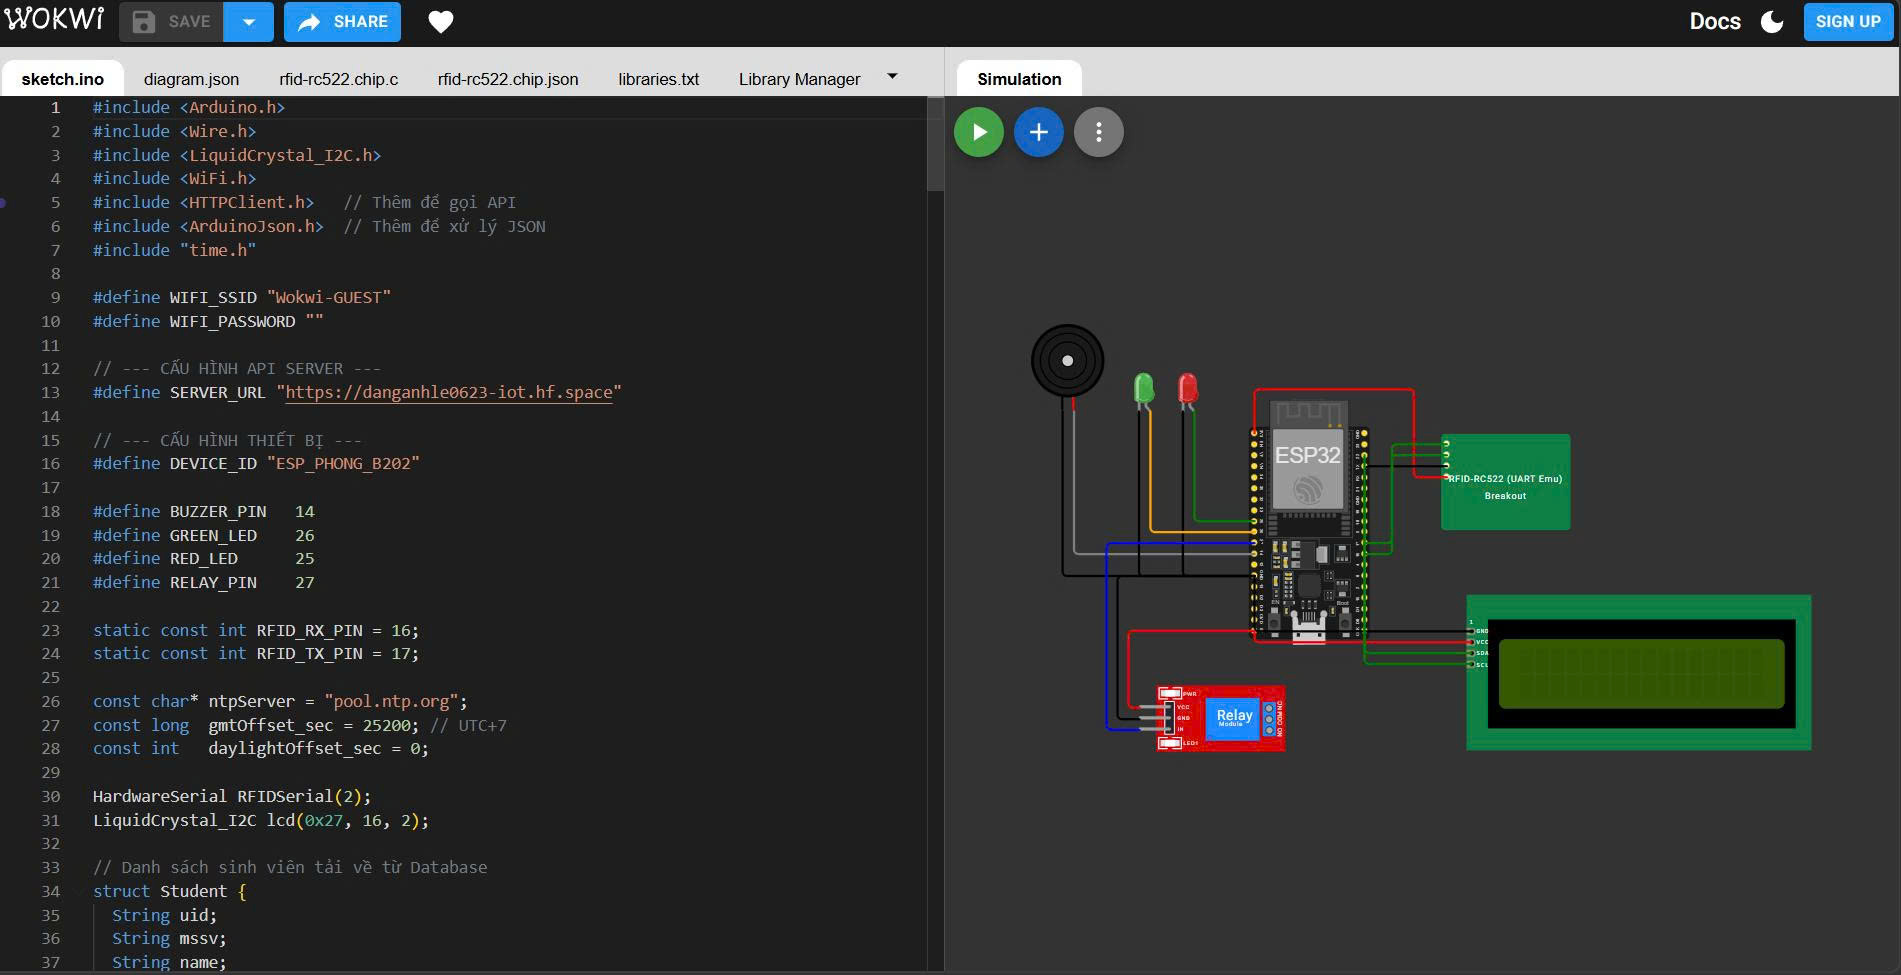
\includegraphics[width=1\textwidth]{img/wokwi.jpg}
    \caption{Ảnh Project trên Wokwi}
\end{figure}

\begin{figure}[h]
    \centering
    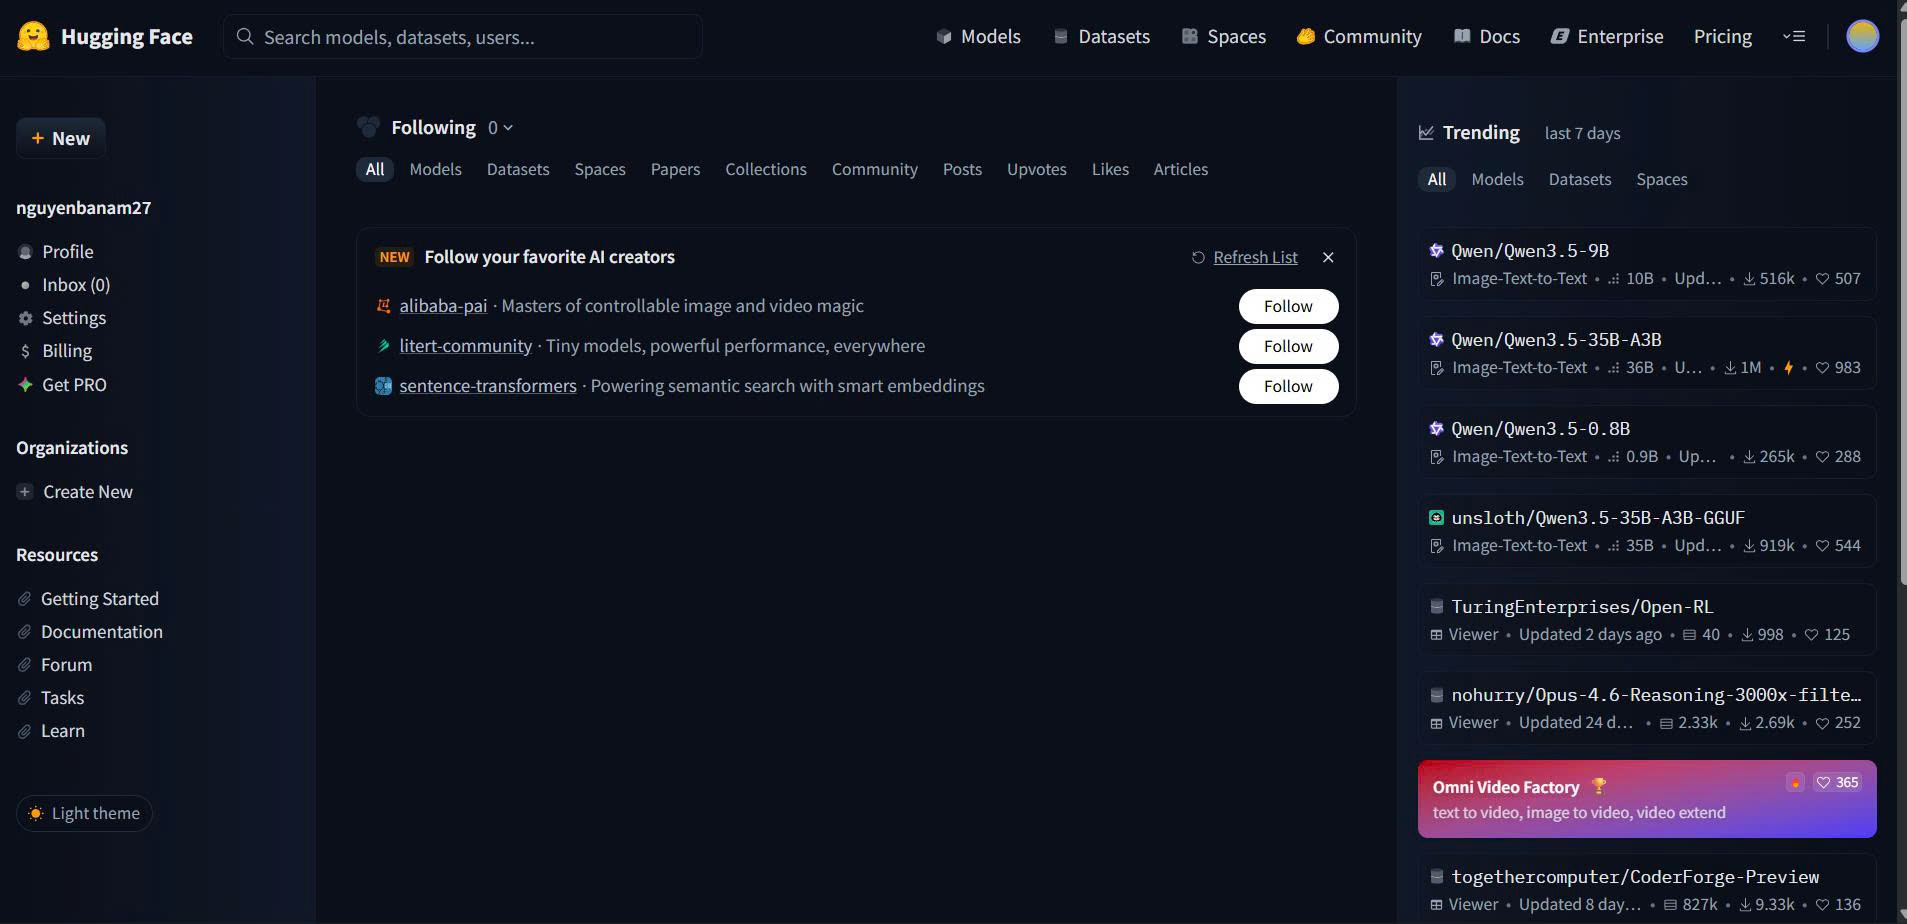
\includegraphics[width=1\textwidth]{img/hugging_face.jpg}
    \caption{Nền tảng Hugging Face}
\end{figure}

\begin{figure}[h]
    \centering
    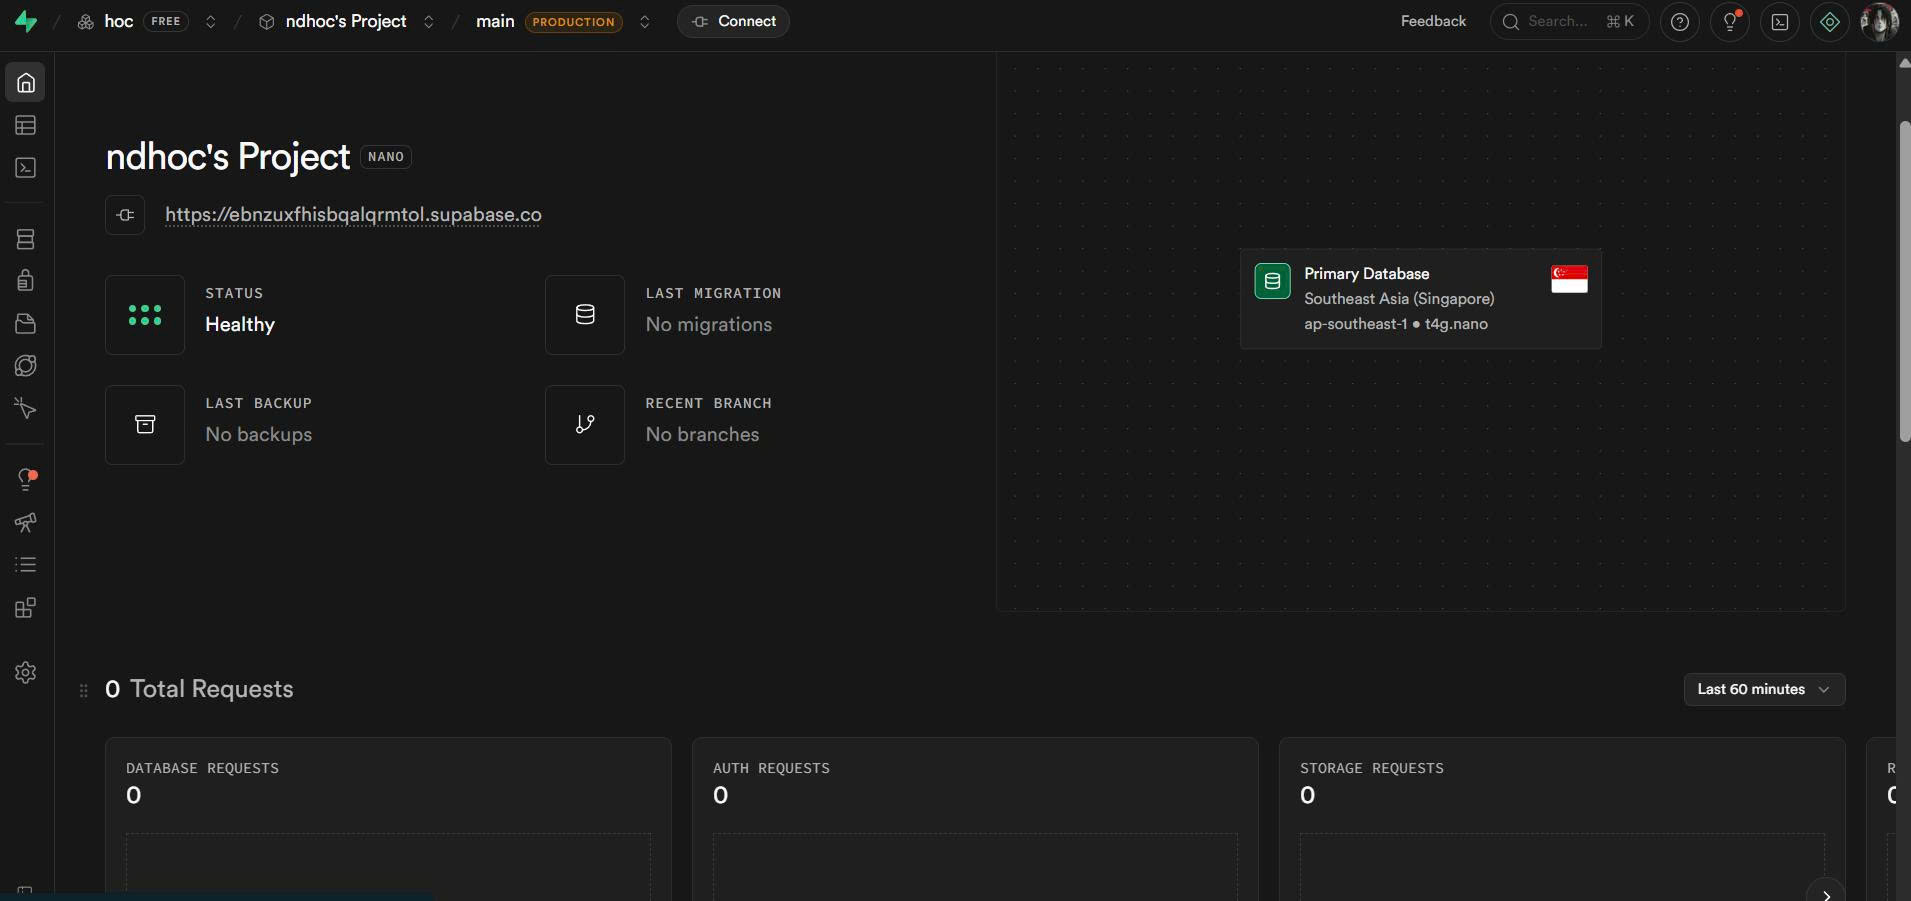
\includegraphics[width=1\textwidth]{img/supabase.jpg}
    \caption{Hệ thống Supabase dùng để lưu trữ Database của project}
\end{figure}

\section{Xây dựng Firmware mô phỏng cho ESP32 trên Wokwi}

Phần Firmware của thiết bị được xây dựng trên nền tảng Arduino IDE với ngôn ngữ lập trình C++. 
Để phục vụ mục đích kiểm thử và mô phỏng phần cứng, hệ thống sử dụng nền tảng Wokwi, cho phép mô phỏng 
hoạt động của vi điều khiển ESP32 cùng các ngoại vi như module RFID, màn hình LCD và các thiết bị 
tín hiệu đầu ra.

Điểm nổi bật của mã nguồn Firmware là việc áp dụng kiến trúc lập trình hướng sự kiện kết hợp với 
cơ chế đa nhiệm của hệ điều hành thời gian thực FreeRTOS. Cách tiếp cận này giúp thiết bị có khả năng 
xử lý đồng thời nhiều tác vụ khác nhau, chẳng hạn như quét thẻ RFID, hiển thị thông tin trên màn hình 
LCD và gửi dữ liệu điểm danh lên máy chủ thông qua mạng Internet.

Nhờ đó, hệ thống có thể duy trì khả năng phản hồi nhanh đối với thao tác quét thẻ của sinh viên, 
đồng thời đảm bảo quá trình truyền dữ liệu lên máy chủ không làm gián đoạn các tác vụ xử lý khác 
của thiết bị.

\subsection{Cấu trúc điều khiển đa nhiệm (FreeRTOS)}

Thay vì sử dụng luồng xử lý tuần tự truyền thống dễ gây tắc nghẽn (Blocking), 
hệ thống sử dụng cơ chế Queue (Hàng đợi) và Task (Tác vụ) riêng biệt để xử lý 
việc truyền dữ liệu lên máy chủ.

\begin{lstlisting}[language=C++, caption={Khởi tạo Queue và Task trong FreeRTOS}]
uploadQueue = xQueueCreate(10, sizeof(UploadData));

xTaskCreatePinnedToCore(
    TaskUpload,    
    "HttpTask",    
    12000,         
    NULL,          
    1,             
    NULL,          
    0              
);
\end{lstlisting}

Việc khởi tạo \texttt{uploadQueue} và \texttt{TaskUpload} giúp tách biệt hoàn toàn 
hai quá trình "Quét thẻ" và "Gửi dữ liệu". Khi sinh viên quẹt thẻ, dữ liệu sẽ được 
đưa vào hàng đợi và phản hồi ngay lập tức trên màn hình LCD. Trong khi đó, quá trình 
gửi yêu cầu POST lên API Server sẽ được Core 0 xử lý ngầm, giúp hệ thống tránh 
bị treo khi phải chờ phản hồi từ mạng Internet.

\subsection{Cơ chế Local Caching và đồng bộ hóa API}

Để giảm độ trễ (Latency) xuống mức thấp nhất (dưới 1 giây), thiết bị ESP32 
không chờ máy chủ xác thực trực tiếp mà thực hiện đối chiếu dữ liệu ngay trên 
danh sách sinh viên đã được tải về bộ nhớ RAM.

\begin{lstlisting}[language=C++, caption={Hàm tải danh sách sinh viên từ API}]
void fetchStudentList() {

    String api_url = String(SERVER_URL) + "/api/students/" + String(DEVICE_ID);

    http.begin(api_url);

    int httpCode = http.GET();

    if (httpCode == HTTP_CODE_OK) {

        for (JsonObject repo : array) {

            students[currentStudentCount].uid = repo["uid"].as<String>();

        }
    }
}
\end{lstlisting}

Hàm này thực hiện truy vấn dữ liệu từ cơ sở dữ liệu Supabase thông qua 
RESTful API khi thiết bị khởi động và được cập nhật lại định kỳ sau mỗi 
30 phút. Nhờ đó, ESP32 có thể xác thực danh tính sinh viên trực tiếp trên 
thiết bị mà không cần truy vấn máy chủ liên tục.

Cơ chế này giúp hệ thống vẫn có thể hoạt động ngay cả khi kết nối Internet 
bị gián đoạn trong thời gian ngắn, đóng vai trò như một chế độ dự phòng 
(Offline Mode) cho hệ thống điểm danh.

\subsection{Xử lý logic nhận dạng và phản hồi người dùng}

Quy trình xử lý mã UID từ module RFID được thiết kế chặt chẽ để tránh việc ghi nhận trùng lặp trong thời gian ngắn.

\begin{lstlisting}[language=C++]
if (line == lastUid && millis() - lastScanMs < 2000) return; // anti spam card

bool found = false;

for (int i = 0; i < currentStudentCount; i++) {
    if (line.equals(students[i].uid)) {
        accessGranted(line, students[i]); // access granted
        found = true;
        break;
    }
}

if (!found) accessDenied(line); // access denied
\end{lstlisting}

Thuật toán kiểm tra \texttt{lastUid} giúp loại bỏ các tín hiệu quét lặp lại trong vòng 2 giây.

Hàm \texttt{accessGranted()} và \texttt{accessDenied()} điều khiển các ngoại vi như Buzzer, LED và Relay để thông báo trạng thái. Dữ liệu sau đó được đóng gói thành định dạng JSON chuẩn trước khi đẩy vào hàng đợi Queue để gửi lên máy chủ.

\subsection{Đồng bộ thời gian thực qua NTP}

Để dữ liệu điểm danh có giá trị pháp lý và chính xác cho việc hậu kiểm, ESP32 thực hiện đồng bộ thời gian với các máy chủ thời gian trên Internet.

\begin{lstlisting}[language=C++]
const char* ntpServer = "pool.ntp.org";

configTime(gmtOffset_sec, daylightOffset_sec, ntpServer);

pkg.timestamp = getEpochTime();
\end{lstlisting}

Hệ thống sử dụng giao thức NTP để lấy thời gian dạng Epoch Time. Việc này đảm bảo rằng mỗi bản ghi điểm danh đều kèm theo nhãn thời gian thực (\textit{Timestamp}), giúp Backend có thể đối soát chính xác với thời khóa biểu được lưu trữ trong cơ sở dữ liệu PostgreSQL.

\section{Xây dựng Backend}

\subsection{Tổng quan kiến trúc Backend}

Trong hệ thống IoT, Backend đóng vai trò là ``bộ não'' trung tâm, chịu trách nhiệm xử lý logic nghiệp vụ, kết nối cơ sở dữ liệu và cung cấp các giao diện lập trình ứng dụng (RESTful API) cho cả thiết bị phần cứng (ESP32) và giao diện Web quản trị.

Hệ thống Backend trong đề tài được xây dựng dựa trên các công nghệ cốt lõi sau:

\begin{itemize}
\item \textbf{Ngôn ngữ và Framework:}  
Sử dụng ngôn ngữ Python với framework FastAPI. FastAPI được lựa chọn nhờ tốc độ xử lý luồng cao nhờ cơ chế lập trình bất đồng bộ (Asynchronous), tích hợp sẵn chuẩn OpenAPI để tự động sinh tài liệu API, đồng thời hỗ trợ xác thực dữ liệu mạnh mẽ thông qua thư viện Pydantic.

\item \textbf{Cơ sở dữ liệu:}  
Sử dụng nền tảng Supabase -- cung cấp hệ quản trị cơ sở dữ liệu quan hệ mã nguồn mở PostgreSQL trên nền tảng đám mây. Hệ thống sử dụng thư viện \texttt{supabase-py} để tương tác trực tiếp với cơ sở dữ liệu.

\item \textbf{Bảo mật và Xác thực:}  
Hệ thống tích hợp cơ chế xác thực JSON Web Token (JWT) với thuật toán mã hóa HS256 để bảo vệ các Endpoint dành cho giao diện Web quản trị. Đồng thời sử dụng thư viện \texttt{passlib} để thực hiện băm (hashing) mật khẩu giảng viên nhằm tăng cường tính bảo mật.
\end{itemize}

\subsection{Thiết kế cơ sở dữ liệu (Database Schema)}

Để giải quyết bài toán điểm danh linh hoạt theo từng ca học trong môi trường đại học, cơ sở dữ liệu của hệ thống được thiết kế theo mô hình chuẩn hóa với 6 bảng chính. Điểm nổi bật trong thiết kế là sự tách biệt giữa ``Thiết bị'' và ``Lớp học'', hai thành phần này được liên kết động với nhau thông qua thông tin \textit{phòng học} và \textit{thời gian thực}.

Các bảng dữ liệu chính bao gồm:

\begin{itemize}
\item \textbf{Bảng thiet\_bi:}  
Lưu trữ mã định danh của thiết bị ESP32 (\textit{device\_id}) và vị trí lắp đặt (\textit{phong\_hoc}).

\item \textbf{Bảng lop\_hoc:}  
Lưu trữ thông tin môn học, mã giảng viên quản lý (\textit{username\_giang\_vien}), phòng học (\textit{phong\_hoc}), cùng khung thời gian học (\textit{gio\_bat\_dau}, \textit{gio\_ket\_thuc}).  
Ngoài ra bảng còn được cấu hình các tham số như \textit{so\_buoi\_toi\_da} và \textit{ti\_le\_hoan\_thanh} làm cơ sở cho các Trigger tự động đánh giá điều kiện dự thi của sinh viên.

\item \textbf{Bảng sinh\_vien:}  
Lưu trữ thông tin cá nhân của sinh viên cùng với mã định danh thẻ RFID (\textit{uid}) dùng cho việc điểm danh.

\item \textbf{Bảng danh\_sach\_lop:}  
Đây là bảng trung gian thể hiện mối quan hệ \textit{nhiều -- nhiều (Many-to-Many)} giữa bảng \textit{sinh\_vien} và \textit{lop\_hoc}.  
Bảng này lưu trữ số buổi đi học, số buổi vắng và trạng thái chuyên cần (``Được thi'' / ``Chưa được thi''). Các trạng thái này được tính toán tự động thông qua các Trigger chạy ngầm trong hệ quản trị cơ sở dữ liệu PostgreSQL.

\item \textbf{Bảng nhat\_ky\_diem\_danh:}  
Lưu trữ toàn bộ lịch sử quét thẻ RFID của sinh viên. Bảng này đóng vai trò như nhật ký hệ thống (Audit Logs), phục vụ việc đối soát dữ liệu với các trạng thái như \textit{Present} (hợp lệ), \textit{Guest} (thẻ lạ) hoặc \textit{Manual Update} (chỉnh sửa thủ công từ giao diện Web).
\end{itemize}

\subsection{Xây dựng các API giao tiếp với ESP32}

Đây là nhóm API quan trọng nhất, đóng vai trò cầu nối dữ liệu giữa thiết bị phần cứng IoT và hệ thống lưu trữ đám mây.

\textbf{API Khởi tạo và đồng bộ danh sách sinh viên (GET /api/students/\{device\_id\})}

Để ESP32 có thể hoạt động ổn định và phản hồi tức thì mà không cần chờ Server xác thực từng thẻ, thiết bị sẽ gọi API này mỗi 30 phút.

\begin{itemize}
\item \textbf{Logic xử lý:}  
Dựa vào \textit{device\_id} truyền lên, Server truy xuất vị trí phòng học của máy quét. Kế tiếp, Server sử dụng đối tượng \textit{datetime} kết hợp múi giờ \textit{VN\_TZ (UTC+7)} để so sánh thời gian hiện tại với \textit{gio\_bat\_dau} và \textit{gio\_ket\_thuc} trong bảng \textit{lop\_hoc}.

\item \textbf{Kết quả:}  
Trả về một mảng JSON gọn nhẹ chứa danh sách \textit{uid}, \textit{mssv} và \textit{name} của lớp học phần đang diễn ra tại thời điểm đó. Nếu là giờ nghỉ, API trả về mảng rỗng để ESP32 chuyển sang chế độ chờ.
\end{itemize}

\textbf{API Xử lý điểm danh theo thời gian thực (POST /api/attendance)}

Khi có sự kiện quét thẻ, ESP32 sẽ đóng gói dữ liệu và gửi yêu cầu POST. Đây là điểm tập trung nhiều luồng xử lý nghiệp vụ phức tạp nhất của Backend.

\begin{itemize}
\item \textbf{Xử lý đồng bộ luồng (Race Condition):}  
Trong môi trường thực tế, sinh viên quét thẻ nối tiếp nhau với tốc độ rất nhanh. Để tránh tình trạng xung đột dữ liệu khi nhiều luồng xử lý của FastAPI cùng ghi vào cơ sở dữ liệu, hệ thống sử dụng cơ chế khóa luồng \texttt{threading.Lock()} của Python thông qua cấu trúc \texttt{with db\_lock:}.  
Cơ chế này buộc các yêu cầu mạng đến gần nhau phải xếp hàng xử lý tuần tự, đảm bảo không bỏ sót bất kỳ gói tin nào.

\item \textbf{Kiểm chứng định danh (Validation):}  
Server trích xuất giá trị \textit{time\_scan} (Epoch time) do ESP32 gửi lên để chuyển đổi về múi giờ Việt Nam, sau đó đối chiếu với mã \textit{uid} của thẻ.

\begin{itemize}
\item \textbf{Trường hợp thẻ hợp lệ:}  
Hệ thống thực hiện lệnh cập nhật tăng số buổi đi học (\textit{so\_buoi\_di\_hoc + 1}) và ghi log với trạng thái \textit{Present}.

\item \textbf{Trường hợp thẻ lạ (Guest):}  
Server không chặn lỗi nhằm tránh làm treo tiến trình xử lý. Thay vào đó, mã thẻ lạ được lưu trực tiếp vào bảng \textit{nhat\_ky\_diem\_danh} kèm trạng thái cảnh báo \textit{Guest}. Sau đó hệ thống vẫn trả về HTTP Code 200 để ESP32 giải phóng hàng đợi dữ liệu.
\end{itemize}

\end{itemize}

\subsection{Xây dựng các API phục vụ quản lý (Web Dashboard)}

Để cung cấp công cụ giám sát trực quan cho giảng viên, Backend cung cấp thêm một nhóm API được bảo mật chặt chẽ.

\begin{itemize}

\item \textbf{Xác thực người dùng (POST /token):}  
Tiếp nhận thông tin đăng nhập của giảng viên, đối chiếu mật khẩu đã được băm bằng thuật toán \textit{bcrypt}, sau đó sinh ra mã thông báo \textit{access\_token} có thời hạn.  
Các API tiếp theo bắt buộc phải truyền Token này thông qua cơ chế \texttt{Depends(get\_current\_user)}.

\item \textbf{Truy xuất thống kê (GET /stats):}  
API này truy xuất danh sách tổng hợp số buổi đi học, số buổi vắng và trạng thái dự thi của toàn bộ sinh viên trong một lớp học cụ thể.

\item \textbf{Xuất báo cáo tự động (GET /export):}  
Hệ thống sử dụng thư viện \textit{pandas} để chuyển đổi dữ liệu từ PostgreSQL thành \textit{DataFrame}, sau đó xuất trực tiếp thành tệp Excel (.xlsx).  
Giải pháp này giúp giảng viên tiết kiệm đáng kể thời gian tổng hợp điểm chuyên cần cuối kỳ.

\item \textbf{Cập nhật dữ liệu thủ công (POST /update-attendance):}  
Cho phép giảng viên chủ động cộng hoặc trừ số buổi đi học trực tiếp trên giao diện Web trong các trường hợp đặc biệt như sinh viên quên thẻ hoặc thiết bị quét gặp sự cố.  
Mọi thao tác đều được hệ thống ghi log dưới nhãn \textit{WEB\_MANUAL} để phân biệt với dữ liệu quét thẻ từ ESP32, đảm bảo tính minh bạch của hệ thống.

\end{itemize}

\section{Xây dựng giao diện Web}

Phần giao diện người dùng (Frontend) đóng vai trò là cầu nối giữa giảng viên hoặc nhà quản trị với cơ sở dữ liệu của hệ thống điểm danh. Giao diện được thiết kế hướng tới các tiêu chí: tốc độ tải trang nhanh, khả năng tương thích với nhiều kích thước màn hình (Responsive), và trải nghiệm người dùng trực quan, hiện đại.

\subsection{Lựa chọn công nghệ và kiến trúc Frontend}

Thay vì sử dụng các thư viện hoặc framework nặng như ReactJS hay VueJS, hệ thống ưu tiên sử dụng HTML5, CSS3 và JavaScript thuần (Vanilla JS).  
Quyết định này giúp trang web có dung lượng rất nhẹ và dễ dàng triển khai trên mọi nền tảng lưu trữ tĩnh (Static Hosting) mà không cần cấu hình phức tạp.

Về mặt thiết kế giao diện (UI), hệ thống áp dụng phong cách thiết kế \textit{Glassmorphism} (hiệu ứng kính mờ) kết hợp với các biến CSS (\textit{CSS Variables}) được định nghĩa trong thẻ \texttt{:root}.  
Việc sử dụng CSS Variables cho phép hệ thống quản lý màu sắc tập trung và hỗ trợ tính năng chuyển đổi giao diện \textit{Light/Dark Mode} một cách linh hoạt.

\subsection{Xây dựng trang xác thực người dùng}

Bảo mật dữ liệu là yếu tố quan trọng khi xây dựng hệ thống quản lý. Do đó, toàn bộ trang chủ được bảo vệ bởi lớp xác thực người dùng.

\begin{itemize}

\item \textbf{Về mặt giao diện:}  
Form đăng nhập được đặt ở vị trí trung tâm của trang với hiệu ứng đổ bóng (\textit{box-shadow}) kết hợp hiệu ứng làm mờ nền (\textit{backdrop-filter: blur}).

\item \textbf{Về mặt trải nghiệm người dùng (UX):}  
Khi người dùng nhập sai thông tin đăng nhập, khung đăng nhập sẽ xuất hiện hiệu ứng rung lắc (\textit{shakeError}) kèm theo viền đỏ nhằm thu hút sự chú ý, thay vì chỉ hiển thị một thông báo lỗi đơn giản.

\item \textbf{Về mặt xử lý logic (JavaScript):}  
Hàm \texttt{handleLogin()} tiếp nhận thông tin tài khoản và mật khẩu, đóng gói dữ liệu vào đối tượng \texttt{URLSearchParams} và gửi yêu cầu POST tới API \textit{/token}.  
Nếu xác thực thành công, Server trả về một mã \textit{JWT (JSON Web Token)}. Mã này được lưu trữ trong \textit{localStorage} của trình duyệt để duy trì phiên đăng nhập cho các lần truy cập tiếp theo.

\end{itemize}

\begin{figure}[htbp]
    \centering
    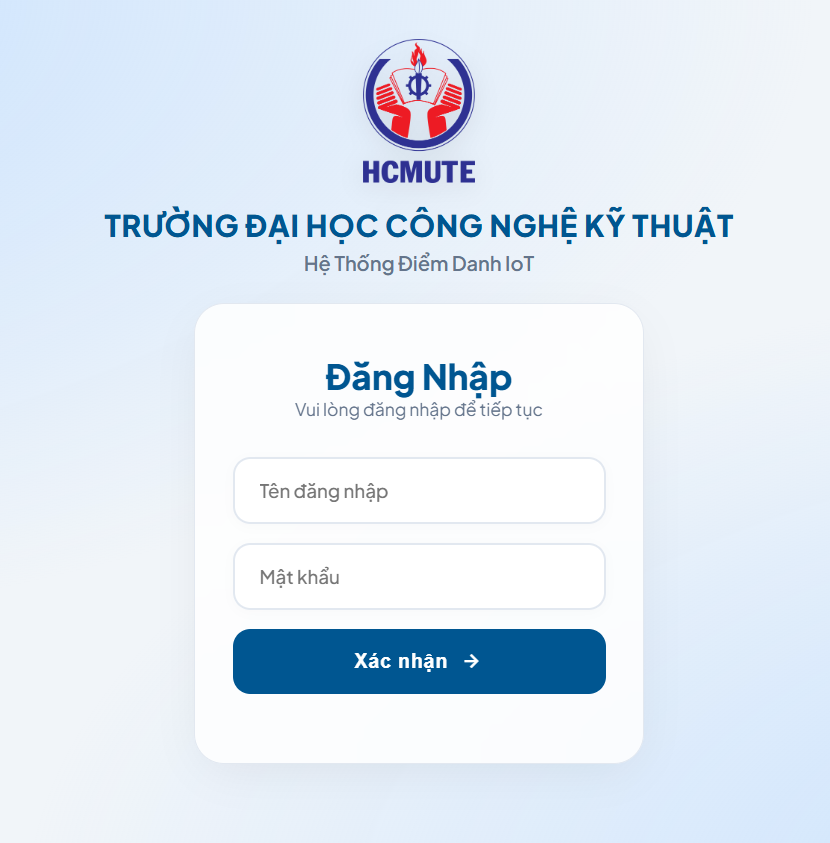
\includegraphics[width=0.6\textwidth]{img/login.png}
    \caption{Giao diện đăng nhập}
\end{figure}
\FloatBarrier

\begin{figure}[htbp]
    \centering
    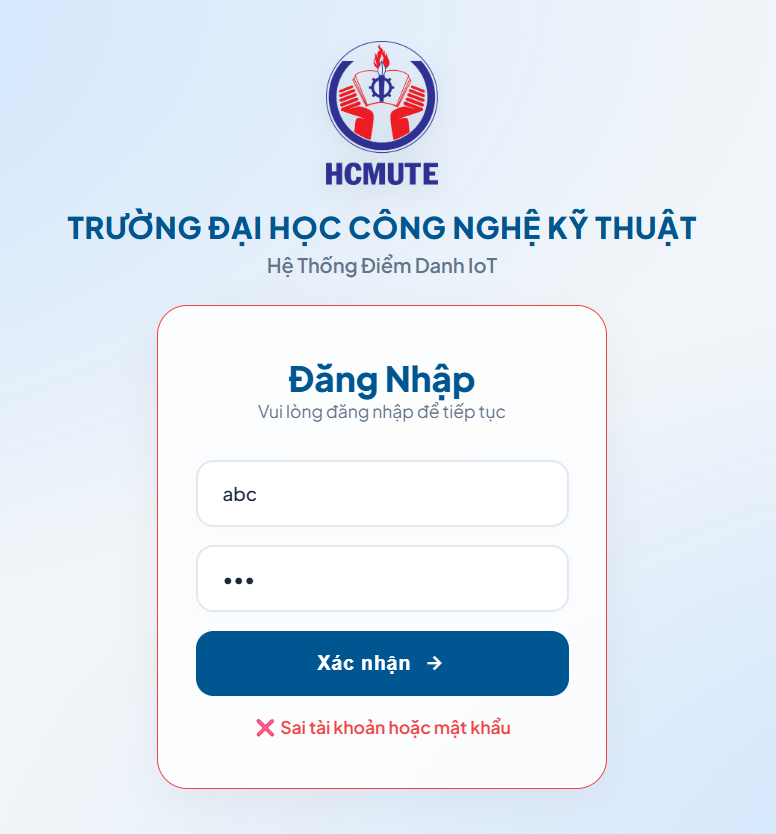
\includegraphics[width=0.6\textwidth]{img/error_login.png}
    \caption{Giao diện khi người dùng nhập sai tài khoản hoặc mật khẩu}
\end{figure}
\FloatBarrier

Đoạn mã để kiểm tra tài khoản hoặc mật khẩu của người dùng nhập vào có hợp lệ hay không được trình bày trong đoạn mã sau:

\begin{lstlisting}[language=JavaScript]
async function handleLogin() {
    try {
        const response = await fetch(`${BASE_URL}/token`, {
            method: "POST",
            headers: { "Content-Type": "application/x-www-form-urlencoded" },
            body: formData
        });

        if (!response.ok) 
            throw new Error("Sai tai khoan hoac mat khau");

        const data = await response.json();

        // Luu token vao bo nho cuc bo
        localStorage.setItem("access_token", data.access_token);

        showDashboard();

    } catch (err) {
        triggerShake();
        errorMsg.innerText = "X" + err.message;
    }
}
\end{lstlisting}

\subsection{Xây dựng Bảng điều khiển (Dashboard) và Quản lý lớp học}

Sau khi xác thực thành công, giao diện Dashboard sẽ được hiển thị thông qua lệnh \texttt{classList.remove("hidden")}. Dashboard được chia thành ba khu vực chính:

\begin{itemize}

\item \textbf{Thanh điều hướng (Top Navbar):}  
Hiển thị tên giảng viên (được lấy từ \texttt{LocalStorage}), nút chuyển đổi chủ đề giao diện (Theme Toggle) và nút Đăng xuất.

\item \textbf{Khu vực điều khiển:}  
Bao gồm một danh sách thả xuống \texttt{<select>} chứa các lớp học do giảng viên phụ trách. Hàm \texttt{loadClasses()} sẽ tự động gọi API \texttt{/my-classes} (kèm theo Token trong Header) để lấy danh sách này ngay khi người dùng truy cập vào trang Dashboard. Bên cạnh đó là các nút thao tác nhanh như \textit{Làm mới dữ liệu} và \textit{Xuất Excel}.

\item \textbf{Khu vực hiển thị và thống kê:}  
Hiển thị nhanh tổng số sinh viên của lớp và số sinh viên thuộc diện cảnh báo học vụ (chẳng hạn như \textit{Cấm thi} hoặc \textit{Chưa được thi}). Ngoài ra, bảng dữ liệu (\textit{Table}) sẽ liệt kê chi tiết thông tin từng sinh viên. Các trường dữ liệu quan trọng như ``Vắng'' được hiển thị bằng màu đỏ nhằm thu hút sự chú ý. Cột ``Trạng thái'' sử dụng các thẻ \textit{badge} với màu sắc khác nhau như \texttt{badge-danger} hoặc \texttt{badge-success} để giúp giảng viên nhanh chóng nắm bắt tình hình lớp học chỉ qua một cái nhìn.

\end{itemize}

\begin{figure}[htbp]
    \centering
    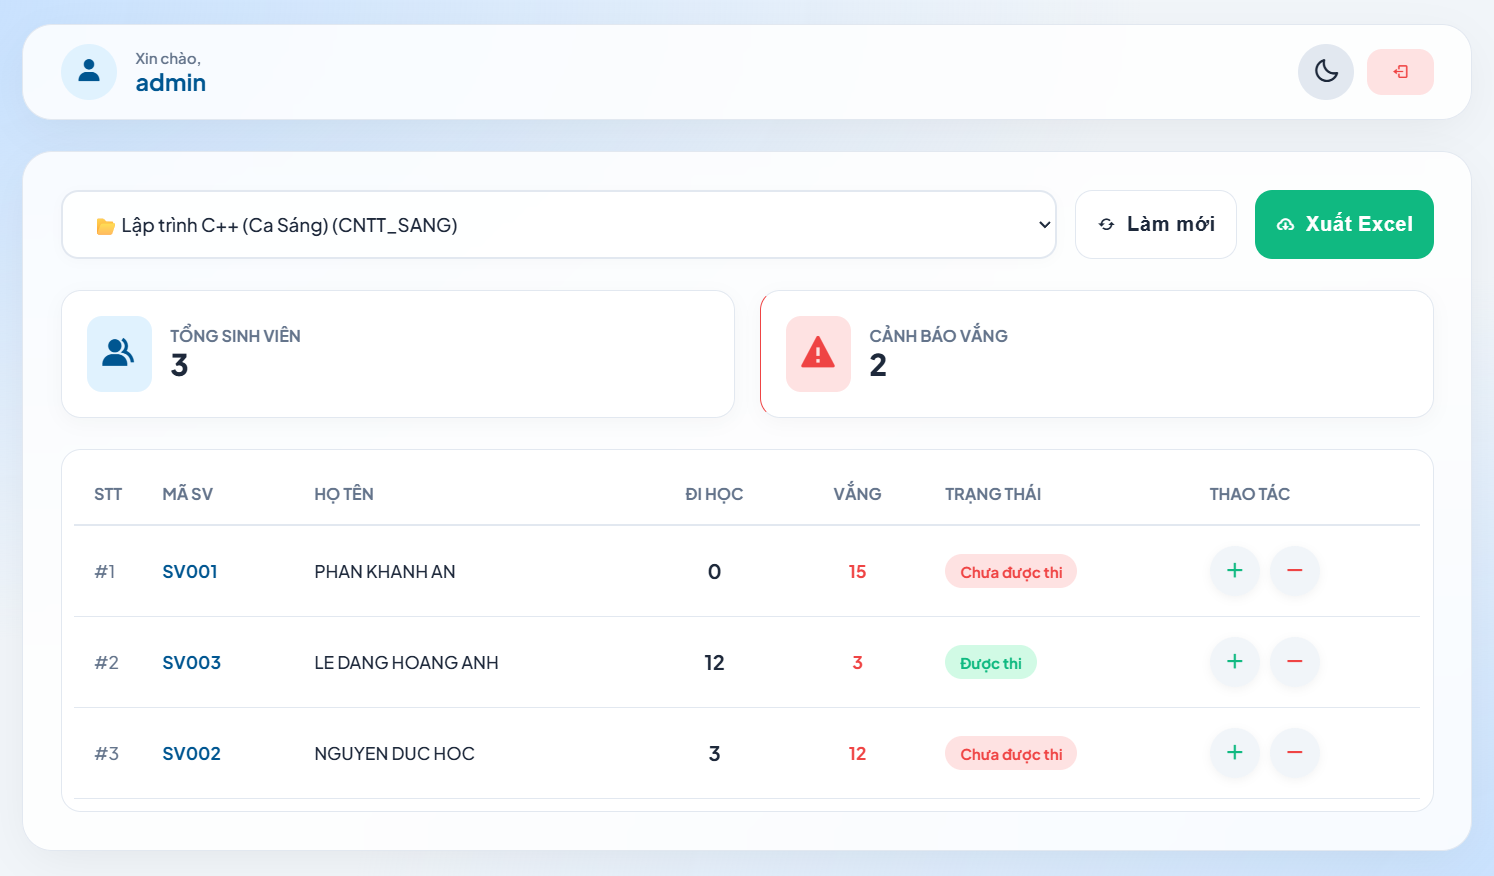
\includegraphics[width=0.9\textwidth]{img/dashboard.png}
    \caption{Giao diện dashboard}
\end{figure}
\FloatBarrier

\subsubsection{Tối ưu hóa Trải nghiệm người dùng (Advanced UI/UX)}

Để hệ thống web đạt tiêu chuẩn của một ứng dụng quản lý hiện đại (Web App), hệ thống không sử dụng các hộp thoại cảnh báo mặc định của trình duyệt (\texttt{alert}, \texttt{confirm}) vì chúng gây gián đoạn luồng công việc (blocking) và có tính thẩm mỹ kém. Thay vào đó, nhóm thiết kế đã tự xây dựng các thành phần giao diện người dùng riêng.

\begin{itemize}
    \item \textbf{Hệ thống Custom Modal:} Khi giảng viên nhấn nút cộng/trừ điểm danh thủ công, một màn hình phủ mờ (\texttt{modal-overlay}) sẽ xuất hiện với hiệu ứng phóng to (\texttt{scaleUp}). Mọi thao tác đều được gán các \textit{callback function}, giúp quá trình xác nhận trở nên an toàn và chuyên nghiệp hơn.



\begin{figure}[htbp]
    \centering
    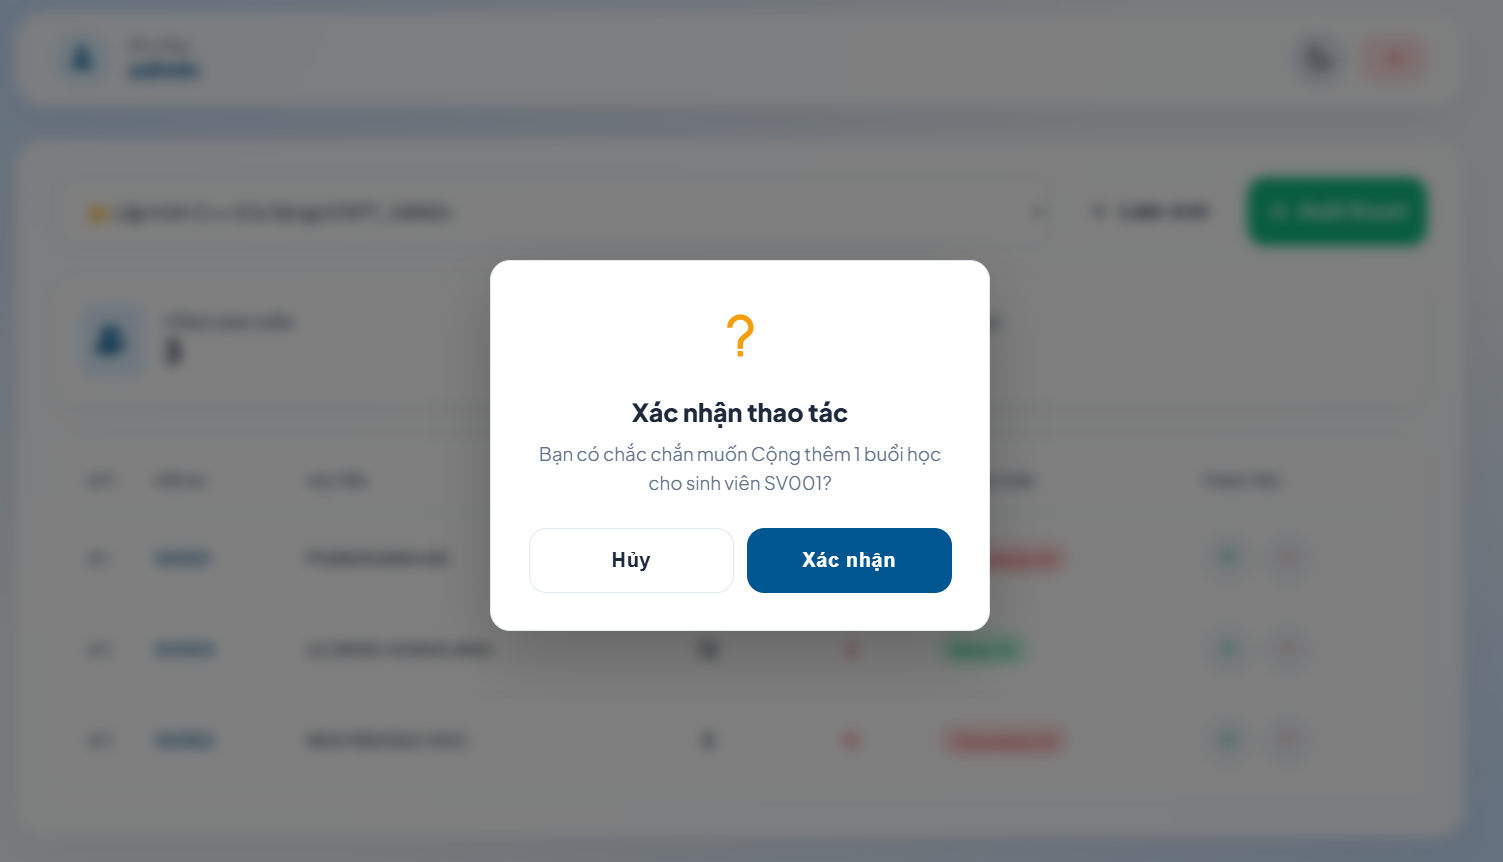
\includegraphics[width=0.9\textwidth]{img/confirm.png}
    \caption{Hộp thoại hiện lên khi giảng viên muốn điểm danh bù cho sinh viên}
\end{figure}
\FloatBarrier

\item \textbf{Hệ thống Toast Notification:} Các thông báo của hệ thống (ví dụ như ``Đăng nhập thành công'', ``Cập nhật dữ liệu lỗi'') được hiển thị dưới dạng cửa sổ pop-up nhỏ (Toast) tại góc dưới bên phải màn hình. Toast sẽ tự động trượt vào màn hình thông qua hiệu ứng \texttt{transform: translateX(0)} và tự động biến mất sau khoảng 3 giây mà không yêu cầu người dùng phải tắt thủ công.

\begin{figure}[htbp]
    \centering
    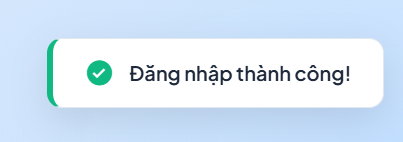
\includegraphics[width=0.7\textwidth]{img/sucessful_login.png}
    \caption{Hộp thoại hiện lên khi đăng nhập thành công}
\end{figure}
\FloatBarrier

\item \textbf{Chế độ nền tối (Dark Mode):} Hệ thống tận dụng thuộc tính \texttt{data-theme} trên thẻ \texttt{<html>}. Khi người dùng nhấn vào nút chuyển đổi biểu tượng mặt trăng/mặt trời, JavaScript sẽ thay đổi giá trị của thuộc tính này thành \texttt{dark} hoặc \texttt{light}. Khi đó toàn bộ các biến CSS được định nghĩa trước sẽ tự động thay đổi, giúp giao diện của toàn bộ trang web chuyển sang chế độ tối hoặc sáng mà không cần tải lại trang. Tùy chọn này cũng được lưu trữ trong \texttt{localStorage} của trình duyệt để hệ thống có thể ghi nhớ thiết lập giao diện của người dùng cho những lần truy cập sau.

\begin{figure}[htbp]
    \centering
    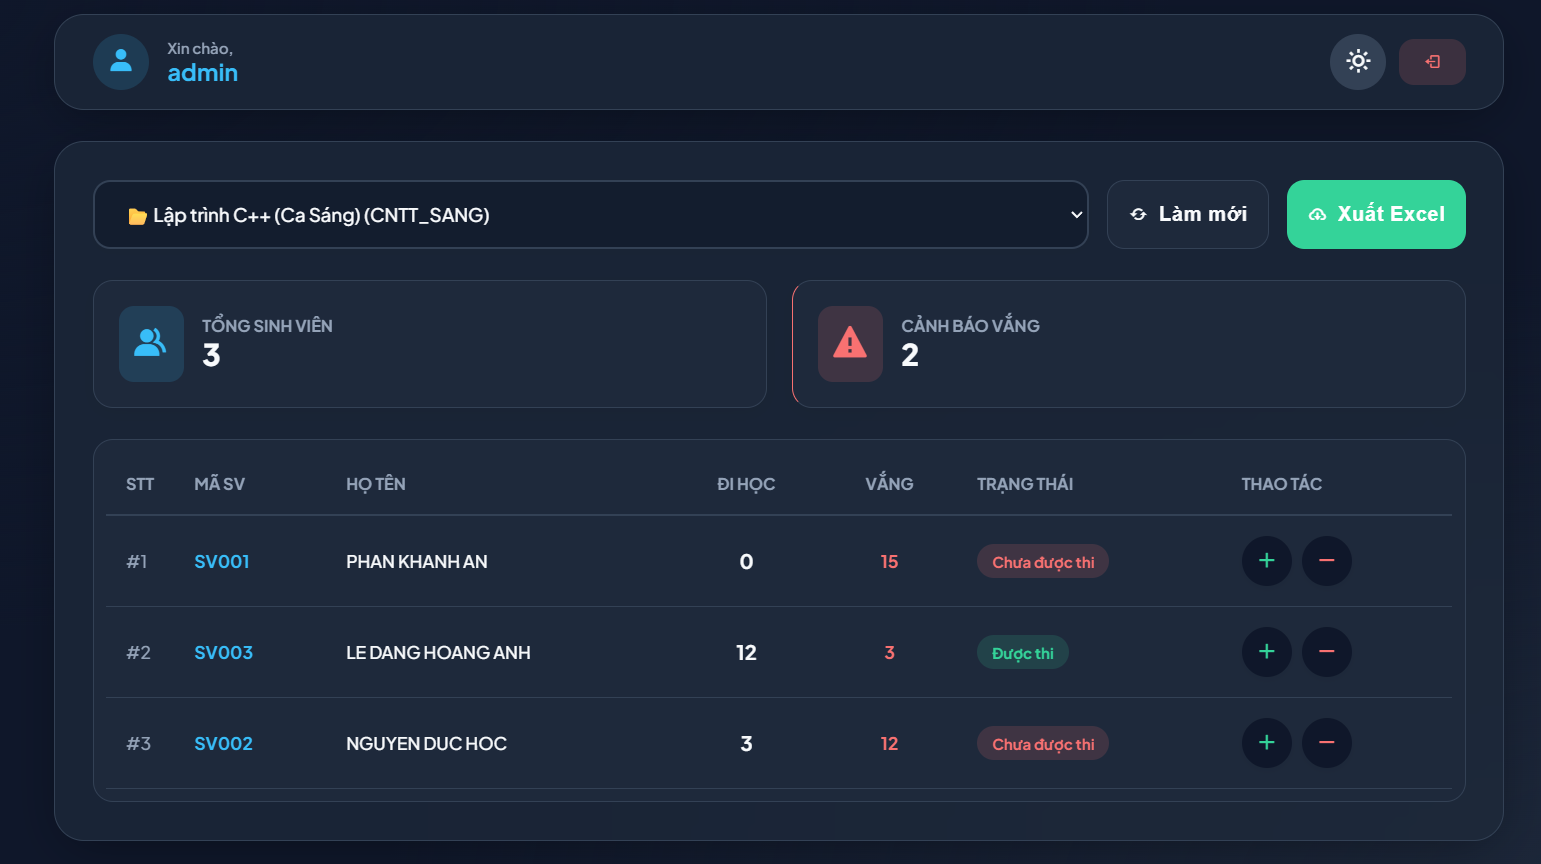
\includegraphics[width=0.9\textwidth]{img/darkmode.png}
    \caption{Giao diện Darkmode}
\end{figure}
\FloatBarrier


\end{itemize}

\subsection{Cơ chế tương tác API và Cập nhật dữ liệu thời gian thực}

Trang web được xây dựng theo mô hình SPA (Single Page Application – Ứng dụng trang đơn) ở mức bán phần. Điều này có nghĩa là khi giảng viên thực hiện các thao tác như lựa chọn lớp học khác hoặc làm mới dữ liệu, trang web không cần tải lại toàn bộ nội dung (reload), giúp trải nghiệm sử dụng trở nên mượt mà và liên tục.

Hàm \texttt{getStats()} sử dụng \texttt{fetch()} API để gửi yêu cầu lấy dữ liệu từ Backend. Trong thời gian chờ phản hồi từ mạng, hệ thống hiển thị một biểu tượng tải dữ liệu (\texttt{bx-loader-alt bx-spin}) nhằm thông báo cho người dùng rằng hệ thống đang xử lý yêu cầu.

Ngoài ra, hệ thống còn hỗ trợ giảng viên can thiệp điểm danh thủ công trong các trường hợp đặc biệt như sinh viên quên mang thẻ RFID. Hàm \texttt{executeEditAttendance()} sẽ gửi một gói tin JSON chứa mã số sinh viên (MSSV) cùng với hành động cần thực hiện (Cộng hoặc Trừ điểm danh) đến máy chủ. Ngay sau khi Server phản hồi thành công (\texttt{response.ok}), hàm \texttt{getStats()} sẽ được gọi lại một cách tự động để cập nhật lại dữ liệu hiển thị trên bảng mà không làm gián đoạn trải nghiệm của người dùng.

\textbf{Tích hợp báo cáo tự động:} Tính năng xuất báo cáo Excel được triển khai thông qua sự phối hợp giữa Backend và Frontend. Khi người dùng nhấn nút ``Xuất Excel'', Frontend sẽ gửi yêu cầu đến Server để lấy file dữ liệu dạng nhị phân (\textit{blob}). Sau đó, JavaScript sử dụng hàm \texttt{window.URL.createObjectURL()} để tạo một đường dẫn tạm thời và giả lập thao tác nhấp chuột tải xuống, cho phép tệp báo cáo định dạng \texttt{.xlsx} được lưu trực tiếp về máy của giảng viên.

\begin{thebibliography}{99}

\bibitem{ref1}
Phạm Quang Huy, Lê Cảnh Trung (2020).
\textit{Lập trình điều khiển với NodeMCU ESP8266 \& ESP32}.
Nhà xuất bản Thanh Niên.

\bibitem{ref2}
Bộ Khoa học và Công nghệ (2019).
\textit{Xu hướng công nghệ Internet of Things (IoT) và ứng dụng trong xây dựng Đô thị thông minh}.
Tạp chí Khoa học và Công nghệ Việt Nam.

\bibitem{ref3}
Espressif Systems (2023).
\textit{ESP32 Technical Reference Manual (Version 5.1)}.
[Online]. Available: \url{https://www.espressif.com/en/support/documents/technical-documents}

\bibitem{ref4}
NXP Semiconductors (2016).
\textit{MFRC522: Standard performance MIFARE and NTAG frontend - Data Sheet}.
Rev. 3.9.  
[Online]. Available: \url{https://www.nxp.com/docs/en/data-sheet/MFRC522.pdf}

\bibitem{ref5}
Klaus Finkenzeller (2010).
\textit{RFID Handbook: Fundamentals and Applications in Contactless Smart Cards, Radio Frequency Identification and Near-Field Communication}.
3rd Edition. John Wiley \& Sons.

\bibitem{ref6}
ISO/IEC (2018).
\textit{ISO/IEC 14443-3:2018 - Cards and security devices for personal identification — Contactless proximity objects — Part 3: Initialization and anticollision}.
International Organization for Standardization.

\bibitem{ref7}
Real Time Engineers Ltd (2023).
\textit{FreeRTOS™ Reference Manual}.  
[Online]. Available: \url{https://www.freertos.org/}

\bibitem{ref8}
Sebastián Ramírez (2023).
\textit{FastAPI Documentation: High performance, easy to learn, fast to code, ready for production}.  
[Online]. Available: \url{https://fastapi.tiangolo.com/}

\bibitem{ref9}
The PostgreSQL Global Development Group (2023).
\textit{PostgreSQL 15 Documentation: Multi-Version Concurrency Control (MVCC) and Transaction Isolation}.  
[Online]. Available: \url{https://www.postgresql.org/docs/}

\bibitem{ref10}
Supabase Inc. (2023).
\textit{Supabase Architecture and PostgreSQL Documentation}.  
[Online]. Available: \url{https://supabase.com/docs}

\bibitem{ref11}
Python Software Foundation (2023).
\textit{Threading — Thread-based parallelism (Python 3.11 Documentation)}.  
[Online]. Available: \url{https://docs.python.org/3/library/threading.html}

\bibitem{ref12}
Benoit Blanchon (2023).
\textit{ArduinoJson 6 Documentation: Efficient JSON serialization for embedded C++}.  
[Online]. Available: \url{https://arduinojson.org/}

\end{thebibliography}

\end{document}